\documentclass[sn-nature]{sn-jnl}% Style for submissions to Nature Portfolio journals

%%%% Standard Packages
\usepackage{graphicx}%
\usepackage{multirow}%
\usepackage{amsmath,amssymb,amsfonts,amsthm,mathrsfs}%
\usepackage[title]{appendix}%
\usepackage{xcolor}%
\usepackage{textcomp}%
\usepackage{manyfoot}%
\usepackage{booktabs}%
\usepackage{algorithm}%
\usepackage{algorithmicx}%
\usepackage{algpseudocode}%
\usepackage{listings}%
\usepackage{tikz-cd}
\usepackage[most]{tcolorbox}
\usepackage{natbib}
\usepackage{fancyhdr}
\usepackage{array}
\usepackage{tabularx}
\usepackage{ragged2e}
\usepackage{adjustbox}
\usepackage{csquotes}
\usepackage{listings}
\usepackage{wrapfig}
\lstdefinelanguage{NetLogo}{
  keywords={to, to-report, end, let, if, else, ifelse, report, foreach, while, loop},
  comment=[l]{;},
  morecomment=[s]{/*}{*/},
  morestring=[b]",
}

\lstset{%
  language=NetLogo,
  basicstyle=\ttfamily\small,
  commentstyle=\color{olive},
  keywordstyle=\color{blue},
  stringstyle=\color{red},
  breaklines=true,
  breakatwhitespace=true,
  tabsize=3,
}
\newcommand{\sbt}{\,\begin{picture}(-1,1)(-1,-3)\circle*{3}\end{picture}\ }



%%%%

%%%%%=============================================================================%%%%
%%%%  Remarks: This template is provided to aid authors with the preparation
%%%%  of original research articles intended for submission to journals published 
%%%%  by Springer Nature. The guidance has been prepared in partnership with 
%%%%  production teams to conform to Springer Nature technical requirements. 
%%%%  Editorial and presentation requirements differ among journal portfolios and 
%%%%  research disciplines. You may find sections in this template are irrelevant 
%%%%  to your work and are empowered to omit any such section if allowed by the 
%%%%  journal you intend to submit to. The submission guidelines and policies 
%%%%  of the journal take precedence. A detailed User Manual is available in the 
%%%%  template package for technical guidance.
%%%%%=============================================================================%%%%

%\jyear{2021}%

%% as per the requirement new theorem styles can be included as shown below
\theoremstyle{thmstyleone}%
\newtheorem{theorem}{Theorem}%  meant for continuous numbers
%\newtheorem{theorem}{Theorem}[section]% meant for sectionwise numbers
%% optional argument [theorem] produces theorem numbering sequence instead of independent numbers for Proposition
\newtheorem{proposition}[theorem]{Proposition}% 
%\newtheorem{proposition}{Proposition}% to get separate numbers for theorem and proposition etc.

\theoremstyle{thmstyletwo}%
\newtheorem{example}{Example}%
\newtheorem{remark}{Remark}%

\theoremstyle{thmstylethree}%
\newtheorem{definition}{Definition}%

\raggedbottom
%%\unnumbered% uncomment this for unnumbered level heads

\begin{document}

\title{Biomimetic Replicant Theory (BRT)}
\subtitle{\large Harmonizing Collaboration, Competition, and Conservation in Knowledge Management}

%%=============================================================%%
%% Prefix	-> \pfx{Dr}
%% GivenName	-> \fnm{Joergen W.}
%% Particle	-> \spfx{van der} -> surname prefix
%% FamilyName	-> \sur{Ploeg}
%% Suffix	-> \sfx{IV}
%% NatureName	-> \tanm{Poet Laureate} -> Title after name
%% Degrees	-> \dgr{MSc, PhD}
%% \author*[1,2]{\pfx{Dr} \fnm{Joergen W.} \spfx{van der} \sur{Ploeg} \sfx{IV} \tanm{Poet Laureate} 
%%                 \dgr{MSc, PhD}}\email{iauthor@gmail.com}
%%=============================================================%%

\author {\fnm{Nathan S.} \sur{Rischling}}
%\hyperlink{mailto:nsr2143@columbia.edu}}%[nsr2143@columbia.edu]{mailto:nsr2143@columbia.edu}}

\affil {\orgname{\normalsize Columbia University}, \orgaddress{\city{\normalsize New York}, \state{\normalsize NY}, \postcode{\normalsize 10027}, \country{\normalsize USA}}}

%%==================================%%
%% sample for unstructured abstract %%
%%==================================%%

\abstract{In complex organizational settings, achieving a harmonious balance between collaboration, competition, and conservation becomes paramount. This research introduces the Biomimetic Resource Theory (BRT) as a framework to elucidate the challenges and opportunities inherent in striking this balance, especially in the realm of knowledge sharing. The BRT emphasizes an organization’s capabilities and advocates a shift from function to intent, fostering a bidirectional relationship where insights drive data discovery just as powerfully as data yields insights. Drawing parallels between natural systems and organizational ecosystems, the BRT offers a comprehensive perspective on sustainable growth and long-term viability in organizational knowledge management. By understanding the dynamics of knowledge flow within the contexts of collaboration, competition, and shifting equilibriums, we can refine knowledge management practices, promoting adaptability and sustainability within these three intertwined dimensions.}

\keywords{Knowledge Management, Category Theory, Constructor Theory, Systems Ecology, Fractal Geometry, Nature-inspired Optimization, Digital Twins, System Resilience, Dynamic Equilibrium}

\maketitle
\pagestyle{fancy}
\fancyhf{} % clear existing header/footer entries
% We don't need to specify the O coordinate
\fancyhead[R]{Rischling BRT Draft v25}
\pagenumbering{arabic}
\fancyfoot[R]{\thepage}
%%================================%%
%% Sample for structured abstract %%
%%================================%%

% \abstract{\textbf{Purpose:} The abstract serves both as a general introduction to the topic and as a brief, non-technical summary of the main results and their implications. The abstract must not include subheadings (unless expressly permitted in the journal's Instructions to Authors), equations or citations. As a guide the abstract should not exceed 200 words. Most journals do not set a hard limit however authors are advised to check the author instructions for the journal they are submitting to.
% 
% \textbf{Methods:} The abstract serves both as a general introduction to the topic and as a brief, non-technical summary of the main results and their implications. The abstract must not include subheadings (unless expressly permitted in the journal's Instructions to Authors), equations or citations. As a guide the abstract should not exceed 200 words. Most journals do not set a hard limit however authors are advised to check the author instructions for the journal they are submitting to.
% 
% \textbf{Results:} The abstract serves both as a general introduction to the topic and as a brief, non-technical summary of the main results and their implications. The abstract must not include subheadings (unless expressly permitted in the journal's Instructions to Authors), equations or citations. As a guide the abstract should not exceed 200 words. Most journals do not set a hard limit however authors are advised to check the author instructions for the journal they are submitting to.
% 
% \textbf{Conclusion:} The abstract serves both as a general introduction to the topic and as a brief, non-technical summary of the main results and their implications. The abstract must not include subheadings (unless expressly permitted in the journal's Instructions to Authors), equations or citations. As a guide the abstract should not exceed 200 words. Most journals do not set a hard limit however authors are advised to check the author instructions for the journal they are submitting to.}



%%\pacs[JEL Classification]{D8, H51}

%%\pacs[MSC Classification]{35A01, 65L10, 65L12, 65L20, 65L70}
\clearpage
\tableofcontents
\listoftables
\listoffigures
\clearpage

\section{Introduction}\label{sec1}

In an era marked by rapid technological advancements and heightened complexities in organizational structures, the quest for optimizing knowledge management has gained unprecedented urgency. Traditionally, the disciplines of biology, mathematics, and organizational behavior have operated in isolated silos. However, this research aims to bridge these diverse fields, offering an integrated lens through which to view and solve problems in contemporary knowledge management. In doing so, it caters to a transdisciplinary audience, transcending the boundaries of any single academic field.

The reader will embark on a journey that commences with the principles governing natural ecosystems, as derived from biomimetic studies. From there, the exploration will delve into mathematical theories capable of formalizing these principles into actionable insights. The culmination of this journey lies in applying these synthesized principles to the realm of organizational behavior and knowledge management. In essence, the voyage undertaken in this paper is from the natural world to mathematical abstraction, and finally, to practical organizational applications.

\subsection{Scope of the Paper}\label{sec1.1}

The following sections are designed to guide the reader through this intricate web of interrelated disciplines. Section~\ref{sec3} provides a comprehensive literature review that lays the groundwork for the Biomimetic Replicant Theory (BRT). Section~\ref{sec4} introduces the theoretical underpinnings of BRT, followed by Section~\ref{sec5} which elucidates the methodology employed for empirical validation. Section~\ref{sec6} presents the results and discussions, and Section~\ref{sec9} offers practical recommendations based on the findings. Finally, Section~\ref{sec10} outlines avenues for future work and potential interdisciplinary collaborations.

This paper aims not merely to introduce a new framework but to catalyze a paradigm shift in how knowledge management is perceived and practiced, influenced by insights from nature and formalized through mathematical rigor.



\section{Background}\label{sec2}

In the intricate world of organizational dynamics, three elements emerge as paramount in shaping outcomes: collaboration, competition, and conservation. Each of these elements, while distinct, intertwines in ways that influence the trajectory of organizations, especially in the realm of knowledge sharing.

Collaboration is the bedrock of innovation\cite{faems_interorganizational_2005}\cite{gonzalez_impact_2003}\cite{ndibu_muntu_keba_kebe_variables_2019}. It is through the collaborative efforts of individuals, teams, and even organizations that new ideas germinate, mature, and come to fruition. The sharing of knowledge, insights, and expertise fuels the collaborative engine, enabling entities to build upon collective wisdom and push the boundaries of what's possible. Yet, as essential as collaboration is, it is not without its challenges. The very act of sharing knowledge can expose vulnerabilities, create dependencies, and sometimes blur the lines of ownership and credit.

Competition, while often perceived as the antithesis of collaboration, plays a vital role in driving excellence. In the quest for resources, market share, or dominance in innovation, competition spurs organizations to optimize, innovate, and adapt. However, it is a double-edged sword. While competition can lead to breakthroughs and advancements, it can also foster secrecy, territorial behaviors, and a reluctance to share knowledge, especially if that knowledge is deemed a competitive advantage\cite{dimitriades_creating_2005}.

Underpinning both collaboration and competition is the principle of conservation. In biological ecosystems, conservation ensures the sustainability and balance of resources, species, and interactions. Similarly, in organizational settings, conservation pertains to the mindful management of knowledge, resources, and relationships. It's about ensuring that in the pursuit of growth, innovation, and dominance, the foundational elements that sustain an organization are not compromised.

This triad of collaboration, competition, and conservation is not static. It exists in a state of dynamic equilibrium, constantly influenced by internal and external factors\cite{nash_equilibrium_1950}. Traditional models of organizational management often struggle to capture this dynamic interplay, leading to gaps in understanding and sub-optimal strategies\cite{nash_non-cooperative_1951}.

Enter the realm of biomimicry. Nature, with billions of years of evolutionary trial and error, offers a treasure trove of insights and solutions\cite{benyus_biomimicry_2009}. From the symbiotic relationships in mycorrhizal networks to the intricate balance of predator-prey dynamics, nature showcases strategies that can inspire organizational approaches\cite{fricker_mycelium_2017}\cite{horton_mycorrhizal_2015}\cite{guichard_meta-ecosystem_2021}. The Biomimetic Resource Theory (BRT) draws from these natural paradigms, offering a framework that melds ecological wisdom with organizational needs\cite{ujwary-gil_organizational_2020}.

Furthermore, to structure and understand the complex relationships within and between these elements, mathematical frameworks such as category theory come into play. Rooted in abstract algebra, category theory provides tools to dissect, analyze, and model intricate systems, making it a fitting companion to the ecological inspirations of the BRT\cite{spivak_category_2014}\cite{fong_invitation_2019}.

In summary, the backdrop against which the BRT operates is one of complexity, dynamism, and interdependence. By understanding the foundational dynamics of collaboration, competition, and conservation, and by drawing insights from nature and mathematical theory, the stage is set to delve deeper into the intricacies of the BRT and its implications for knowledge management in organizational settings.
\section{Literature Review}\label{sec3}
\subsection{Gödel's Incompleteness Theorems and Their Implications for Systems Theory (Zalta et al., 2020)\cite{zalta_gos_2020}}
\paragraph{Summary}
Kurt Gödel's incompleteness theorems, first published in 1931, have had a profound impact on the field of logic, mathematics, and even philosophy. The theorems essentially argue that for any consistent formal system capable of performing a certain level of arithmetic, there will be statements that are neither provable nor disprovable within the system. This revelation has had a ripple effect, challenging traditional notions of completeness, consistency, and even the limits of human knowledge.

\paragraph{Core Concepts}
Gödel’s theorems rely on a few foundational concepts:

\textbf{Formal System:} A set of axioms with rules of inference, designed for mechanically generating new theorems.

\textbf{Consistency:} A formal system is consistent if it doesn't result in contradictory conclusions.

\textbf{Completeness:} A system is complete if, for every statement, either the statement or its negation can be derived.

These concepts resonate strongly with elements in systems theory, particularly when discussing complex systems' predictability and comprehensibility.

\paragraph{First Incompleteness Theorem}
The first theorem states that any consistent formal system, where a certain amount of elementary arithmetic can be performed, is incomplete. This theorem doesn't just make a claim; it also provides a method to generate specific "undecidable" statements. This finding has implications for any system striving for a holistic understanding, including biological, social, and computational systems.

\paragraph{Second Incompleteness Theorem}
The second theorem extends the first by stating that a consistent formal system cannot prove its own consistency. This self-referential limitation has significant parallels in systems theory, particularly when contemplating self-regulating systems. It poses questions about the limits of self-awareness in complex systems, a subject also examined in biomimicry and cybernetic systems.

\paragraph{Applicability Beyond Arithmetic}
While Gödel's theorems were formulated in the context of arithmetic, their scope extends to any system where a modicum of arithmetic can be performed. This makes the theorems highly relevant to a variety of disciplines, including computer science and artificial intelligence, where questions about system limitations are pervasive.

\paragraph{Exceptions and Limitations}
It is essential to note that not all systems are incomplete. For instance, Presburger arithmetic is both complete and decidable. However, any system that integrates both addition and multiplication of integers falls under the purview of Gödel's theorems, making them relevant for most scientific models that involve computation or formal logic.

\paragraph{Conclusion}
Gödel's incompleteness theorems offer a sobering view of the limitations inherent in formal systems, an insight that has ramifications far beyond the realm of mathematics. For researchers in systems theory, these theorems provide a rigorous framework for discussing system boundaries and the limits of completeness and consistency. They serve as a valuable touchstone for contemplating complex systems' intricate, often paradoxical, nature.

\subsection{Developing A Cost Overrun Predictive Model For Complex Systems Development Projects (Adoko, 2015)\cite{adoko_developing_2015}}

Project cost overrun, especially in large-scale endeavors, has been a consistent area of research and analysis. The challenges of project management, combined with unpredictable factors, often result in financial discrepancies from initial projections. Moses Tawiah Adoko, in "Developing A Cost Overrun Predictive Model For Complex Systems Development Projects," addresses this issue by proposing a predictive methodology.

Adoko's work provides a systematic overview of existing literature on cost estimation methodologies. Previous models, primarily deterministic in nature, encountered challenges when applied to the multifaceted contexts of expansive projects.

In response, "Developing A Cost Overrun Predictive Model For Complex Systems Development Projects" introduces a statistical methodology. Utilizing modern statistical techniques, Adoko presents a structured approach to data collection, validation, and model training, emphasizing the need for accurate prediction in complex scenarios.

A central component of Adoko's research is the analysis of prior models. These models, varying in their focus from detailed insights to broader trends, displayed adaptability challenges in dynamic environments. Adoko's findings suggest that while these models provided foundational insights, there was room for enhancement in terms of adaptability.

Another noteworthy aspect of Adoko's research is the consideration of the human element in project management. The research suggests that while quantitative models form the base, human decision-making, biases, and perceptions have a role in the eventual project outcomes. Adoko's methodology seeks to incorporate both quantitative and qualitative elements to create a holistic model for predicting cost overruns.

To conclude, "Developing A Cost Overrun Predictive Model For Complex Systems Development Projects" offers a structured approach to the issue of cost overrun prediction. The research synthesizes past methodologies, identifies gaps, and proposes a comprehensive model, positioning it as a relevant contribution to the literature on complex systems, project management, and financial prediction.
\subsection{Non-Cooperative Games (Nash, 1951)\cite{nash_non-cooperative_1951}}
In the realm of game theory, the understanding of non-cooperative games has been fundamentally advanced by John Nash's seminal paper titled "Non-Cooperative Games" published in 1951. This work provides a systematic exploration of situations where players make decisions independently, without the possibility of enforceable collaboration or collusion.

Nash's paper introduces the concept of equilibrium for non-cooperative games. This equilibrium, now widely known as the Nash Equilibrium, describes a situation in which each player's strategy is optimal, given the strategies chosen by all other players. In this state, no player has an incentive to unilaterally change their strategy, assuming the strategies of the other players remain unchanged.

The methodology employed by Nash is rooted in mathematical rigor. Utilizing fixed-point theorems, Nash demonstrates the existence of equilibrium in games, even when players employ mixed strategies that involve randomization. This finding contrasts with earlier understandings of game theory, which were primarily centered around pure strategies.

Furthermore, Nash delves into the distinction between cooperative and non-cooperative games. While cooperative games allow for enforceable agreements between players, non-cooperative games, as addressed in this paper, operate under the premise that such binding agreements are absent. This distinction is vital for the application of game theory in various real-world scenarios, especially in economics and social sciences.

One of the standout features of Nash's research is its applicability across a spectrum of disciplines. While the immediate context is mathematical and theoretical, the implications of Nash's equilibrium concept extend to economics, political science, and even biology, providing a foundational framework for understanding strategic interactions in diverse settings.

In conclusion, John Nash's "Non-Cooperative Games" represents a pivotal contribution to the field of game theory. By introducing and rigorously proving the concept of Nash Equilibrium, this work reshaped the understanding of strategic interactions in non-cooperative contexts and has left an indelible mark on subsequent research in the field.
\subsection{Category Theory for Scientists (Spivak, 2014)\cite{spivak_category_2014}}

In "Category Theory for Scientists," David I. Spivak embarks on a comprehensive exploration of category theory, tailored specifically for the scientific community. The work stands as a notable attempt to elucidate the foundational principles of this mathematical domain in an accessible manner.

At its core, Spivak's exposition centers around key tenets of category theory, such as objects, morphisms, and functors. These concepts, while foundational to the field, are often presented in contexts that may appear abstract or detached from empirical practices. Spivak addresses this gap by contextualizing these principles within the realm of scientific applications.

The work is structured in a manner that integrates theoretical discussions with practical examples, enhancing its relevance to a broader audience. While maintaining the rigor expected of mathematical literature, Spivak ensures that the content remains approachable by providing clear explanations and drawing parallels to familiar scientific concepts.

A distinguishing feature of the book is its pedagogical framework. The inclusion of exercises and interactive elements serves a dual purpose. Firstly, it offers readers an opportunity for hands-on engagement with category theory principles. Secondly, it reinforces understanding by allowing readers to apply the learned concepts in varied contexts.

In summation, "Category Theory for Scientists" presents a structured and objective exploration of category theory. By bridging the gap between abstract mathematical constructs and their practical implications in science, Spivak's work contributes to the existing literature and offers a valuable resource for interdisciplinary research.
\subsection{Constructor Theory of Information (Deutsch and Marletto, 2015)\cite{deutsch_constructor_2015}}

In "Constructor Theory of Information," David Deutsch and Chiara Marletto embark on a profound exploration of the intersection between constructor theory and the concept of information. This work stands as a significant contribution to the ongoing discourse on the foundational principles of physics, particularly in the context of quantum theory and information dynamics.

The crux of the paper revolves around the proposition that information is a central and indivisible element of the physical universe. Deutsch and Marletto argue that traditional views on information, while foundational, may have overlooked the intricate interplay between information and the laws of physics. They advocate for a reconceptualization of information through the lens of constructor theory.

A distinguishing aspect of the research is the rigorous methodology employed. The authors present a theoretical framework that integrates constructor theory, a set of principles proposed by Deutsch that seeks to explain all physical processes in terms of possible and impossible tasks, with the dynamics of information. This fusion results in a novel perspective on the nature of information and its relation to physical reality.

The paper also delves into the implications of this theoretical framework, particularly in the context of quantum mechanics. The authors provide insights into the challenges posed by quantum phenomena and offer potential solutions grounded in the constructor theory of information.

In conclusion, "Constructor Theory of Information" by Deutsch and Marletto presents a paradigm shift in the understanding of information within the realm of physics. By integrating constructor theory with the dynamics of information, the authors pave the way for a deeper understanding of the universe's fundamental principles. Their work is a notable addition to the academic literature, offering fresh perspectives and stimulating further research in the field.
\subsection{Organizational Development and Change Theory: Managing Fractal Organizing Processes (Henderson \& Boje, 2016)\cite{henderson_organizational_2016}}

In "Organizational Development and Change Theory: Managing Fractal Organizing Processes", Henderson and Boje delve deeply into the intricate dynamics of organizational development and the inherent challenges of change management. This seminal work serves as an exploration into the multifaceted nature of organizations, emphasizing the concept of fractal organizing processes.

Central to the paper's narrative is the assertion that organizational structures and processes, akin to fractals in nature, exhibit patterns that repeat at varying scales. Henderson and Boje argue that understanding these recursive patterns is pivotal for effective organizational development and change management.

The research methodology is comprehensive, intertwining theoretical constructs with empirical observations. By amalgamating insights from systems theory, complexity theory, and organizational behavior, the authors present a holistic view of organizational dynamics.

A standout feature of the paper is its emphasis on the practical implications of fractal organizing processes. Henderson and Boje offer actionable insights for practitioners, suggesting strategies and interventions that align with the inherent fractal nature of organizations. This pragmatic orientation ensures the work's relevance to both academic scholars and professionals engaged in organizational development.

Furthermore, the paper juxtaposes traditional organizational theories with the proposed fractal perspective, shedding light on the potential advantages and challenges of the fractal approach.

In summation, "Organizational Development and Change Theory: Managing Fractal Organizing Processes" by Henderson and Boje offers a fresh lens through which to view organizational dynamics.  

\subsection{Biological Relativity Requires Circular Causality but Not Symmetry of Causation: So, Where, What and When Are the Boundaries? (Noble et al., 2019)\cite{noble_biological_2019}}

In "Biological Relativity Requires Circular Causality but Not Symmetry of Causation: So, Where, What and When Are the Boundaries?", Noble and colleagues present a comprehensive exploration of the principles of biological relativity and their implications for understanding causality in biological systems. This work stands at the intersection of biology and theoretical physics, offering a fresh perspective on the intricate dynamics of living organisms.

The crux of the paper revolves around the assertion that biological relativity necessitates a framework of circular causality. Noble et al. challenge traditional linear causal models, highlighting their limitations in capturing the complex interplay of factors within biological systems. The authors emphasize the need for a more nuanced understanding, where causality is viewed as a recursive, interconnected web.

The research methodology employed is characterized by a synthesis of theoretical constructs and empirical observations. Drawing upon principles from both biology and relativity theory, Noble and colleagues weave a narrative that emphasizes the interconnectedness and interdependence of biological entities.

A distinguishing aspect of the paper is its treatment of the concept of symmetry in causation. The authors argue against a symmetrical view of causality, positing that while biological processes exhibit circular causality, they do not necessarily adhere to a symmetrical framework. This distinction is crucial for understanding the boundaries and limitations of biological relativity.

Furthermore, the paper delves into the practical implications of these theoretical constructs. Noble et al. explore the potential applications of their findings, highlighting their relevance for both academic research and practical endeavors in biology and medicine.

In conclusion, "Biological Relativity Requires Circular Causality but Not Symmetry of Causation: So, Where, What and When Are the Boundaries?" by Noble et al. offers a novel perspective on the nature of causality in biological systems. By integrating principles of relativity and biology, the authors present a framework that challenges traditional views and paves the way for a deeper understanding of the intricacies of life.
\subsection{Interorganizational Collaboration and Innovation: Toward a Portfolio Approach (Faems et al., 2005)\cite{faems_interorganizational_2005}}
To understand behaviors at a crossdisciplinary level, the study conducted by Faems et al. (2005), categorized collaboration as an existing quality of organizations and did not decompose the input conditions. They hypothesized organizational intent and overall strategic alignment contribute to the partnerships established for collaborative interactions\cite{faems_interorganizational_2005}. They defined partnerships by comparing research and development (R\&D) relationships with the location, number, and type of participants. Additionally, continued analysis of specific partnerships indicated two overarching motivations: explorative and exploitive. The variable \enquote{$\sigma$-collaborations} was established to measure homogeneous interprofessional collaboration. Each entity received a score of 0 to 7, derived from specific entity types such as customers or universities.  Another variable \enquote{\#Exploitation-oriented collaborations,} scored relationships with customers and suppliers from 0 to 10. Similarly, \enquote{\#Exploration-oriented collaborations} captured collaborations with research institutes or universities on a scale of 0 to 10\cite{faems_interorganizational_2005}. The authors concluded that research-oriented partnerships indicate an explorative relationship to further innovation and knowledge exchange to create something new. Conversely, collaboration with mutually dependent organizations leans toward exploitive motivation to improve an existing interest\cite{faems_interorganizational_2005}. These findings provide relevant insight into the impact of motivation, intent, and alignment on collaborative relationships.

\subsection{The impact of group process variables on the effectiveness of distance collaboration groups (González et al., 2003)\cite{gonzalez_impact_2003}}
González et al. (2003) measured the group behavioral performance, task cohesion, collective efficacy, and interpersonal attraction 71 distance collaboration groups to their distance collaboration effectiveness using two competing models. The first model centered around the hypothesis that proposed group cohesion variables would causally predict group effectiveness from an exogenous position. Alternatively, the authors’ second model hypothesizes that the effectiveness of distance collaboration increases when collective efficacy influences cohesion as the exogenous variable\cite{gonzalez_impact_2003}.

Material to the study is group performance and effectiveness, defined as “behavior or action in which group members engage”\cite{gonzalez_impact_2003}. The remaining variables are products of various observable behaviors and motivations. Each variable was measured using observations from teaching assistants and data from surveys administered to group participants and their peers.

Further insight into the nuanced relationships between selected variables and behavioral inputs was also provided for consideration. Attention is directed to the subjective nature associated with translations of the surveys developed in English and presented in Spanish. Also noted by the authors is the influence of participant behaviors driven by undocumented contextual factors.

Compiled data was analyzed using a structural equation model to convey relevant empirical correlations and statistics shown in table \ref{table:1}.\\ \begin{table}[h]
\centering
\begin{tabular}{l l l l l l l }
\hline
Variable & M & S.D. & 1 & 2 & 3 & 4 \\
\hline
Interpersonal attraction & 5.36 & 1.04 & – & & & \\

Task cohesion & 5.48 & 1.01 & 0.71* & – & & \\

Collective efficacy & 3.86 & 0.59 & 0.60* & 0.75* & – & \\

Team and peer facilitation & 4.55 & 0.82 & -0.02 & -0.03 & -0.06 & – \\

Group effectiveness (quality) & 3.21 & 0.50 & 0.09 & 0.26* & 0.13 & 0.26* \\
\hline
\end{tabular}
\caption{Descriptive statistics and correlations among study variables at the group level of analysis\cite{gonzalez_impact_2003}.}
\label{table:1}
\end{table} 

Then the outputs were fed into both models to test their hypotheses, revealing statistically significant findings.

Relationships between task cohesion, team and peer facilitation, and collective efficacy played a meaningful role in the quality of work achieved. Lastly, the study confirmed the predicted impacts on group effectiveness in distance collaboration scenarios. 


\subsection{How mycorrhizal associations drive plant population and community biology (Tedersoo et al., 2020)\cite{tedersoo_how_2020}}
Common mycelial networks (CMNs) enhance most plants' nutrient access and stress tolerance and mediate plant interactions. Furthermore, several different species of mycorrhizal fungi can be the key determinants of both population and dynamics within plant communities. CMNs mediate relationships between species or individual entities by “promoting the performance of inferior competitors…and suppressing superior competitors”\cite{tedersoo_how_2020}.

Mycelial networks also protect plant populations by acting as a communications relay to send messages from distressed individuals attacked by a pathogen or herbivore. Dependence on mycorrhizal fungi reflected in equalizing and stabilizing mechanisms further extends to soil feedback and properties, carbon nutrient relocation, and trading. Moreover, allocated resources can be prioritized to benefit familial individuals within the network or in a hierarchical manner amongst the same species\cite{tedersoo_how_2020}.

Citing synthesis of available literature, the authors propose CMNs have been a previously unrecognized equalizing variable fostering plant coexistence. Further suggested is long-term community monodominance enabled by synergies between mycorrhizal fungi and plant populations\cite{tedersoo_how_2020}.

Tedersoo et al., (2020) conclude the positive impacts of CMNs on plant communities are evidenced by distinct methods of nutrition observed in certain species residing where nutrient availability is scarce or in areas of extreme environmental conditions. Lastly, the authors propose that species-specific relationships and interactions are worthy of future exploration within the context of resultant diversity, promoting further diversity\cite{tedersoo_how_2020}.

\subsection{Community Assembly and the Functioning of Ecosystems: How Metacommunity Processes Alter Ecosystems Attributes (Leibold et al., 2017)\cite{leibold_community_2017}}

The interplay between community assembly and the functioning of ecosystems is a topic that has long fascinated ecologists. The intricate dynamics that govern the assembly of species and their subsequent interactions influence not only the composition of communities but also the broader functionality of ecosystems. Leibold et al. delve into this intricate relationship, shedding light on the overarching principles and nuances that govern these dynamics.

The cornerstone of Leibold and colleagues' work is the concept of metacommunity processes. By examining communities not as isolated entities but as interconnected elements of larger metacommunities, the authors provide a fresh perspective on the drivers of community assembly and its consequent impacts on ecosystem functioning.

One of the standout features of this research is the rigorous exploration of the various pathways through which metacommunity dynamics influence ecosystem attributes. By mapping these pathways, Leibold et al. offer a structured framework that encompasses both direct and indirect influences, adding depth and granularity to our understanding.

The implications of metacommunity processes on ecosystem functioning are manifold. Leibold and colleagues highlight how species sorting, mass effects, and patch dynamics influence nutrient cycling, productivity, and stability. These insights underscore the intertwined nature of community composition and ecosystem processes, emphasizing the need for holistic approaches in ecological research.

Moreover, the paper astutely recognizes the role of spatial dynamics in shaping metacommunity processes. By integrating spatial factors into their analyses, the authors showcase the importance of considering both spatial and temporal scales in understanding the assembly-function relationship.

In conclusion, "Community Assembly and the Functioning of Ecosystems: How Metacommunity Processes Alter Ecosystems Attributes" stands as a pivotal contribution to the field of ecology. By intertwining the concepts of community assembly, metacommunity dynamics, and ecosystem functionality, Leibold et al. present a comprehensive exploration that enriches our understanding and offers avenues for future research in the realm of community ecology.

\subsection{Variables associated with interprofessional collaboration: The case of professionals working in Quebec local mental health service networks (Ndibu Muntu Keba Kebe et al., 2019)\cite{ndibu_muntu_keba_kebe_variables_2019}}
Ndibu Muntu Keba Kebe et al. performed a secondary analysis on multiple variables to study their relationship with interprofessional collaboration (IPC). Between the four variables selected (individual characteristics, interactional characteristics, organizational features, and professional role characteristics), the authors hypothesized that interactional characteristics and organizational features would have the most relevant relationships with IPC. Sub-traits of interactional characteristics—Team climate, knowledge sharing, knowledge integration, and multifocal identification—emerged as having significant associations with IPC\cite{ndibu_muntu_keba_kebe_variables_2019}.
IPC has gained traction in chronic and mental healthcare settings to improve patient management, with the benefits of improved patient health status and care satisfaction being reported. However, organizational adoption and implementation are still lacking. Within the overarching blocks of variables, individual variables were defined using various instruments, as seen in Table \ref{table:3}.

\begin{table}[h!]
\begin{adjustbox}{center}
\begin{tabularx}{0.9\paperwidth}{p{4.5cm} >{\RaggedLeft\arraybackslash}p{.15cm} >{\RaggedRight\arraybackslash}p{3.2cm} X}
\hline
\textbf{Blocks of variables} & & \textbf{Variables} & \textbf{Instruments} \\
\hline
\multirow{4}{*}{\textbf{IV: Individual Characteristics}} & 1 & Age & Socio-demographic questionnaire. \\
& 2 & Sex & Socio-demographic questionnaire. \\
& 3 & Belief in interdisciplinary benefits & Five-item[\sbt] scale; $\alpha$: 0.92; Range: 5–35 (Sicotte, D’Amour \& Moreault., 2002). \\
& 4 & Team Seniority & Socio-demographic questionnaire. \\
\multirow{8}{*}{\textbf{IV: Interactional Characteristics}} & 5 & Knowledge sharing & Five-item[\sbt] scale; $\alpha$: 0.93; Range: 5–35 (Bock, Zmud, Kim, \& Lee, 2005). \\
& 6 & Knowledge integration & Nine-item[\sbt] scale; $\alpha$: 0.95; Range: 9–63 (Song \& Xies, 2000). \\
& 7 & Team commitment & Four-item[\sbt] scale; $\alpha$: 0.86–0.92; Range: 4–28 (Allen \& Meyer, 1990). \\
& 8 & Decision-making participation & Three-item[\sbt] scale; $\alpha$: 0.88; Range: 3–21 (Campion, Medsker, \& Higgs, 1993). \\
& 9 & Mutual trust & Four-item[\sbt] scale; $\alpha$: 0.90; Range: 4–28 (Simons \& Peterson, 2000). \\
& 10 & Team climate & Nineteen-item[\sbt] scale; $\alpha$: 0.60–0.84; Range: 19–133 (Anderson \& West, 1998). \\
& 11 & Team conflict & Nine-item[\sbt] scale; $\alpha$: 0.93–0.94; Range: 9–63 (Jehn \& Mannix, 2001). \\
& 12 & Team autonomy & Three-item[\sbt] scale; $\alpha$: 0.76; Range: 3–21 (Campion, Medsker \& Higgs, 1993). \\
\multirow{2}{*}{\textbf{IV: Organizational Features}} & 13 & Organizational support & Four-item[\sbt] scale; $\alpha$: 0.84–0.85; Range: 4–28 (Spreitzer, 1996). \\
& 14 & Team size & Socio-demographic questionnaire. \\
\multirow{2}{*}{\textbf{IV: Role Characteristics}} & 15 & Profession type & Socio-demographic questionnaire. \\
& 16 & Multifocal identification & Twelve-item[\sbt] scale; $\alpha$: 0.65; Range: 12–84 (Van Dick et al., 2004). \\
\multirow{1}{*}{\textbf{DV}} & & IPC & Fourteen-item[\sbt] scale: communication (5 items); synchronization (3 items), explicit coordination (3 items); implicit coordination (3 items); $\alpha$: 0.77-0.91; Range: 14–98 (Chiocchio, Grenier, O’Neil, Savaria \& Willms, 2012). \\
\hline
\end{tabularx}
\end{adjustbox}
\caption{Variables and Instruments}
\label{table:3}
\end{table}




In alignment with their hypothesis, the interactional characteristics and organizational features blocks had the strongest link to interprofessional collaboration\cite{ndibu_muntu_keba_kebe_variables_2019}. Finally, Ndibu Muntu Keba Kebe et al. used their results to recommend the following actions for increasing IPC: maintain awareness of potential team degradation, encourage mentorship between new and tenured employees, and leverage activities or training programs that bring awareness to the core skills of interprofessional collaboration \cite{ndibu_muntu_keba_kebe_variables_2019}.

\subsection{Meta-ecosystem dynamics: understanding ecosystems through the transformation and movement of matter (Guichard \& Marleau, 2021)\cite{guichard_meta-ecosystem_2021}}

Diverging from traditional theories of ecosystems and metapopulations, \citet{guichard_meta-ecosystem_2021} put forth meta-ecosystem dynamics as a new model to integrate peripheral areas of research whose interactions were previously treated as incidental with little attention paid to the impacts\cite{guichard_meta-ecosystem_2021}. Expanding on metapopulation and metacommunities theories, the claim is made that feedbacks link biodiversity and ecosystem functions rather than a consequence of degradation. Furthermore, the authors posit interactions between inorganic and organic matter flows contribute to “population growth and species assembly,”\citep[p. v]{guichard_meta-ecosystem_2021} which comprise central components of meta-ecosystem dynamics page.
The theory pursues a multidisciplinary compilation of insights from nonlinear dynamics, applied mathematics, ecology, and non-equilibrium dynamics.

A comprehensive list of variables is provided as a reference for each equation presented. While species interaction and behavior are mentioned, the mathematical expressions convey communities and ecosystems using “stocks and fluxes of energy”\citep[p. 3]{guichard_meta-ecosystem_2021}, providing alternative boundaries to view the represented system. In alignment with their objective, Guichard \& Marleau (2021) empirically demonstrate the nonlinear impacts of cycling and matter movement on communities and ecosystems traditionally unobserved.

Expanding on the Rosenzweig-MacArthur model to include the recycling of matter in a predator-prey relationship, establishing the link to states of non-equilibrium, in contrast to previous notions of linear responses driving a local equilibrium\cite{guichard_meta-ecosystem_2021}. Consistent with the authors’ goals, the underlying proofs and models are the primary method to support their theory, with observational data being immaterial to the overall concept. However, the substituted values demonstrate the intent of meta-ecosystem dynamics with outputs representative of plausible scenarios\cite{guichard_meta-ecosystem_2021}.

Guichard \& Marleau (2021) conclude that concepts introduced by meta-ecosystem dynamics support the “development of a general and inclusive body of theory”\citep[p. 86]{guichard_meta-ecosystem_2021}. Lastly, future research must guide current literature and theoretical ecology principles toward intersectionality.


\section{Methodology}\label{sec4}

The core of this research is underpinned by a rigorous, quantitative methodology that seamlessly marries theoretical constructs with mathematical expressions. This meticulous approach ensures a robust validation of the Biomimetic Replicant Theory (BRT).
\subsection{Research Design}
This study is grounded in the Biomimetic Replicant Theory (BRT), which seeks to understand the intricacies of knowledge flow, competition, and collaboration in organizational ecosystems by drawing parallels with natural systems. Our research framework amalgamates elements of game theory, systems theory, category theory, and biomimicry, serving as a multidisciplinary bridge to explore the dynamics of knowledge management.

\paragraph{Mixed Method Approach} A combined case study and exploratory approach was employed to delve deep into transdisciplinary topics and fields\cite{plano_clark_mixed_2016}.

\paragraph{Secondary Data Analysis} Quantitative data from from cited references were analyzed to draw correlations between natural and human behavioral models and networks\cite{john_sage_2012}. This analysis aimed to uncover similarities between systems, offering insights to enhance organizational knowledge management efforts in support of collaboration, competition, and conservation.
\paragraph{Visualization and Presentation}
Various visualizations, including scatter plots and line graphs, were developed to represent the relationships between variables. These visualizations aided in interpreting the data and drawing concrete conclusions about the dynamics of competition, collaboration, and resource consumption.

\subsection{Data Collection}
\subsubsection{Primary Data}
\paragraph{The GFG Fractal Model}
A novel computational model run in NetLogo\cite{wilensky_netlogo_1999-1}, referred to as the "GFG Fractal" model, was developed to simulate the interactions of entities (represented as turtles) in an environment competing for resources. This model captured key variables such as the number of initial players, maximum resource availability, and initial strategies. The model was iteratively run, producing datasets that reflect the evolution of strategies and resource consumption.

\paragraph{\enquote{WILDFIRE} Network Diffusion Simulation} This simulation, also based on the NetLogo platform\cite{wilensky_netlogo_1997}, provided data on how ideas diffused across the organizational network under varying conditions. Key parameters manipulated in this simulation include \( M_{ij} \), \( \beta_i \), \( t_{jj'} \), and \( \theta \).


\subsection{Theoretical Framework}

\paragraph{Biomimicry Principles} Derived from nature, quantitative patterns and behaviors observed in ecological interactions were extracted to lay the foundational blueprint for the BRT\cite{guichard_meta-ecosystem_2021}.

\paragraph{Category Theory} Serving as a backbone for a structured and quantitative framework, category theory's abstract mathematical depth was harnessed. Used as a foundational tool for drawing parallels between datasets, this approach formalized complex relationships within organizational ecosystems, ensuring a rigorous, quantitative lens for the study. Furthermore, commutative diagrams (Figure \ref{fig:extended_commutative_diagram}) were constructed to showcase the interrelationships and mappings between variables from different datasets, providing a rigorous mathematical basis for comparative analysis\cite{spivak_category_2014}\cite{fong_invitation_2019}.

\begin{figure}[H]
\centering
\begin{tikzcd}[row sep=5.5cm, column sep=6cm]
\text{GFG Variables} 
    \arrow[r, "F", "\begin{array}{c}
                     \text{initial-players} \mapsto \text{Colonization} \\
                     \text{max-resource} \mapsto \text{Nutrient Level} \\
                     \text{initial-strategy} \mapsto \text{Toxicity}
                     \end{array}" description]
    \arrow[d, "G" swap, "\begin{array}{c}
                        \text{mean(strategy)} = f(\text{initial-players, max-resource}) \\
                        \text{mean(payoff)} = g(\text{initial-strategy, max-resource})
                        \end{array}" description]
    \arrow[rd, "N", dashed, "\text{Bootstrapping}" pos=0.2]
& \text{Fungi Variables} 
    \arrow[d, "H", "\begin{array}{c}
                   \text{Colonization} = h(\text{Toxicity, Nutrient Level}) \\
                   \text{Resource Allocation} = k(\text{Colonization, Nutrient Level})
                   \end{array}" description]
    \arrow[ld, "M", dashed, "\text{Transformation}" pos=0.2]
\\
\text{GFG Measures}
    \arrow[r, "I", "\begin{array}{c}
                    \text{mean(strategy)} \mapsto \text{Toxicity} \\
                    \text{mean(payoff)} \mapsto \text{Resource Allocation}
                    \end{array}" description] 
& \text{Fungi Measures}
\end{tikzcd}
\begin{align*}
\boxed{
\begin{aligned}
\textbf{Key:} \\
F & : \text{Functor mapping GFG Variables to Fungi Variables} \\
G & : \text{Mathematical expressions in GFG} \\
H & : \text{Mathematical expressions in Fungi study} \\
I & : \text{Functor mapping GFG Measures to Fungi Measures} \\
N & : \text{Natural transformation representing Bootstrapping in GFG} \\
M & : \text{Natural transformation representing Transformation in Fungi} \\
\end{aligned}
}
\end{align*}
\caption{Extended Commutative Diagram for Methodological Integration: A Category-Theoretic Approach.}
\label{fig:extended_commutative_diagram}
\end{figure}

\subsubsection{Development of the Biomimetic Replicant Theory (BRT)}

Inspired by the quantitative patterns from nature and the analytical tools of category theory, the BRT was formulated using precise mathematical constructs. This structure encapsulated the intricate dynamics of knowledge within organizations.


\subsubsection{Models, Simulations, and Data Analysis}

\paragraph{Model Development} Leveraging mathematical expressions and tools like NetLogo for network-centric modeling, models were developed to quantitatively represent various organizational scenarios.

\paragraph{Simulation Scenarios} Grounded in quantitative methods, simulations were designed to mimic real-world organizational challenges. The performance of BRT-guided strategies was quantitatively assessed against traditional approaches.

\paragraph{Data Analysis with SPSS} Data analysis was conducted using IBM’s SPSS software. Following data cleaning and preparation, a comprehensive analysis was performed, ranging from descriptive statistics to inferential statistics. SPSS Modeler, with its user-friendly interface and robust capabilities, was utilized for predictive modeling, data preprocessing, and extracting insights from unstructured data sources.

\paragraph{Comparative Analysis}
The GFG Fractal data and human cooperation data were juxtaposed to identify parallels in strategy dynamics and resource allocation. Special attention was paid to understanding how both humans and entities in the model respond to shifting conditions and achieve equilibrium in strategy and payoff.

\paragraph{Bootstrapped Regression Trees (BRT) Framework}
A Bootstrapped Regression Trees framework was employed to analyze the GFG Fractal data. This technique allowed for a nuanced understanding of how initial conditions influence mean strategy and payoff values. The BRT framework effectively handled non-linearity and interactions between predictors, ensuring robust and interpretable results.





\subsubsection{Iterative Refinement}

Results from simulations were rigorously analyzed. Any discrepancies between the BRT's mathematical predictions and the simulation outcomes led to iterative refinements, ensuring the BRT's theoretical robustness and practical relevance. Models and primary datasets are avaialble at nrischling.github.io
\subsection{The Biomimetic Replicant Theory: An Overview}
\subsubsection{Definition and Principles}
BRT posits that the most efficient and optimized human-made systems can be derived by mimicking nature's solutions. This is not merely about copying but understanding the foundational principles that make natural systems efficient, resilient, and adaptable\cite{leibold_community_2017}. While innovations like digital twins offer simulations of reality, BRT emphasizes a deeper alignment with nature's design principles\cite{tao_digital_2018}.
\subsection{Three Foundational Laws of BRT}
\subsubsection*{I. Human systems can achieve optimization through mimicry of naturally occurring equivalents }
\paragraph{Optimization through Mimicry}
Nature, over millennia, has refined processes and systems that work harmoniously. Emulating these processes can lead to optimization in human systems\cite{benyus_biomimicry_2009}.
Examples: The streamlined design of trains inspired by bird beaks, and building designs optimized for temperature control modeled after termite mounds.
\subsubsection*{II. No human system will ever surpass the optimization of a corresponding natural
system}
\paragraph{Limitations of Human Optimization}
While we can strive for perfection, our artificial systems will always fall short of their natural counterparts. This is not a limitation of innovation but rather an acknowledgment of the complexities and nuances inherent in natural systems\cite{west_scale_2017}\cite{noble_theory_2012}.
Reasons might include our inability to fully comprehend multi-dimensional interactions in nature, unknown variables, or the sheer efficiency and simplicity of natural processes.
\subsubsection*{III. All human systems are synthetic derivatives of natural systems}
\paragraph{Derivative Nature of Human Systems}
Every human system, at its core, can be traced back to a natural counterpart. This idea challenges us to always seek inspiration from the world around us\cite{odum_ecological_1994}.
For example, the internet can be likened to mycelial networks, and community structures might mimic animal social hierarchies.


\subsection{Generative Fractal Games (GFGs) in the Context of Biomimetic Replicant Theory}
The Generative Fractal Game (GFG) concept within the Biomimetic Replicant Theory offers a profound mechanism to understand complex systems' dynamics, both natural and human-made. This idea is particularly aligned with non-cooperative game theory, where individual players make decisions to maximize their utility without considering the collective good. In this vein, Fujiwara and Greve\cite{fujiwara-greve_non-cooperative_2015} emphasize the non-cooperative nature of games, where players' strategies are defined by their individual goals and constraints, often leading to suboptimal outcomes for the system as a whole.

GFGs echo this sentiment but introduce an added layer of complexity. The fractal nature of GFGs suggests that games are played at multiple scales, with each smaller game contributing to a larger, encompassing game. This mirrors the hierarchical structure observed in many natural systems, where small-scale interactions cumulatively influence large-scale dynamics. However, the generative aspect implies that as these games evolve, they spawn new games, reflecting the dynamic and ever-changing nature of systems\cite{noble_biological_2019}.

\begin{figure}[h]
\centering
\begin{minipage}{0.55\textwidth}  % Increased from 0.5 to 0.55
\centering
\begin{tikzcd}[scale=1.8, row sep=3cm, column sep=3cm]  % Increased scale from 1.5 to 1.8
A \arrow[r, "f", shift left] & C \arrow[l, "g", shift left] \arrow[loop right, "h", looseness=7, out=30, in=330]
 \\
B \arrow[u, "i", shift left] \arrow[ur, "j", swap] & G \arrow[u, "k"] \arrow[l, "l", swap]
\end{tikzcd}
\end{minipage}%
\begin{minipage}{0.35\textwidth}  % Decreased from 0.4 to 0.35
\begin{align*}
\boxed{
\begin{aligned}
\textbf{Key:} \\
A & : \text{Player A} \\
B & : \text{Player B} \\
C & : \text{Combined Player} \\
G & : \text{Game} \\
f & : \text{Strategies} \\
g & : \text{Equilibrium} \\
h & : \text{Evolution} \\
i & : \text{Composition (Player B to Player A)} \\
j & : \text{Composition (Player B to Combined Player)} \\
k & : \text{Composition (Game to Combined Player)} \\
l & : \text{Composition (Game to Player B)}
\end{aligned}
}
\end{align*}
\end{minipage}
\caption[Commutative Diagram of Generative Fractal Games]{Commutative Diagram of Generative Fractal Games (GFGs) in Biomimetic Replicant Theory: A Multi-Scalar Representation of Dynamic Equilibria and Evolutionary Game Mechanics. The diagram illustrates the complex interplay between individual players (A and B), their collective entity (C), and the overarching game structure (G). Arrows represent various relationships such as strategies, equilibrium states, and compositional dynamics, thereby capturing the fractal, generative, and ever-evolving nature of GFGs.}
\label{marker}
\end{figure}

John Nash's pioneering work on equilibria in non-cooperative games offers a foundational pillar for understanding GFGs\cite{arsenyan_modeling_2015}. Nash's equilibrium\cite{nash_equilibrium_1950} represents a state in which no player has an incentive to deviate from their chosen strategy, given the strategies chosen by other players. Within the GFG framework, Nash equilibria can be visualized as points of stability at various scales. However, due to the dynamic and generative nature of these games, these equilibria may shift or evolve, reflecting the inherent instability and incompleteness of systems in equilibrium. This notion of incompleteness aligns with Gödel's incompleteness theorems, which propose that within any consistent formal system, there are truths that cannot be proven or disproven\cite{zalta_gos_2020}. Similarly, BRT posits that true equilibrium in any system, including GFGs, may remain elusive and unprovable, ever-shifting, and evolving.

By integrating Nash's equilibrium concept with the fractal, generative, and incompleteness aspects of GFGs, we can conceptualize a multi-scalar, dynamic system where equilibria at smaller scales contribute to, and are influenced by, equilibria at larger scales. This interplay between scales, the shifting nature of equilibria, and the ever-evolving game dynamics offers a rich tapestry to understand complex systems, whether they be ecological, economic, or organizational.

The GFG offers a fresh perspective, viewing every entity as part of a larger whole, contributing and being shaped by the larger system. This fractal nature echoes in both natural and human-made systems, suggesting a universality in system design and behavior\cite{mandelbrot_fractal_1982}.

\noindent % This ensures there's no indentation at the start of the line
% Begin the first minipage for the diagram




\subsubsection{BRT and the Universe as a Generative Fractal Game}
The universe operates as a vast interconnected network, where every entity, from galaxies to atoms, plays a part in shaping the whole. This idea is mirrored in BRT, where human systems are both players and constituents of a larger game (Guichard, 2021).
\subsubsection{Decomposition of Equilibrium}
In the GFG, strategies are fluid, changing based on the dynamics of the game. This reflects the dynamic equilibrium observed in nature, where entities adapt and evolve based on external pressures\cite{smith_logic_1973}.
Drawing from Gödel's Incompleteness Theorems, we can infer that any state of equilibrium in the GFG is transient and cannot be fully understood or defined while being observed. This introduces a degree of unpredictability and acknowledges the limitations of our understanding\cite{newman_structure_2003}.

\subsubsection{Implications for Systems Understanding}

\paragraph{Nested Hierarchies}
The GFG suggests systems operate within interconnected hierarchies, offering insights into modeling and understanding intricate systems\cite{ujwary-gil_organizational_2020}.
\paragraph{Dynamic Equilibrium} This challenges traditional static models and emphasizes adaptability and responsiveness as key components of system design\cite{holland_hidden_1996}.

\begin{figure}[h]
\centering
\begin{minipage}{0.6\textwidth}
\centering
\begin{tikzcd}[row sep=1.5cm, column sep=1.5cm, cells={nodes={font=\large}}]
B \arrow[r, "F", dashed] \arrow[d, "D_1"', bend right=15, swap]
& F \arrow[d, "R", bend left=15] \\
E \arrow[r, "Seek Guidance", dotted] \arrow[d, "D_2"', bend right=15, swap]
& M \arrow[d, "Learn & Share", dashed, bend left=15, pos=0.3] \\
E_L 
& M_L
\end{tikzcd}
\end{minipage}%
\begin{minipage}{0.4\textwidth}
\begin{align*}
\boxed{
\begin{aligned}
\textbf{Key:} \\
B & : \text{Bee} \\
F & : \text{Selection of Flowers based on Knowledge} \\
D_1 & : \text{Bee's Discernment from vast stimuli} \\
R & : \text{Offering quality resources} \\
E & : \text{Employee} \\
D_2 & : \text{Employee's Discernment from advice} \\
M & : \text{Manager} \\
E_L & : \text{Employee after Learning} \\
M_L & : \text{Manager after Sharing Knowledge} \\
\textbf{---} & : \text{Direct knowledge flow or interaction} \\
\textbf{- - -} & : \text{Discernment process} \\
\textbf{- $\cdot$ -} & : \text{Pattern or method of discernment}
\end{aligned}
}
\end{align*}
\end{minipage}
\caption[Behavioral Fractal Example]{Behavioral Fractal Example illustrating the complex interactions and shared behaviors in knowledge transfer between bees and managers/employees. Both groups navigate a myriad of information sources, requiring discernment to prioritize valuable knowledge and resources\cite{chittka_mind_2022}. Emphasizing quality over quantity, they utilize specific patterns, methods, and interactions to identify and share the most pertinent knowledge.}


\end{figure}



\paragraph{Real-world Analogies}
From market dynamics to ecological systems, the GFG provides a lens through which we can understand and predict system behavior.
\paragraph{Organizational Strategy and Management}
GFG principles can be integrated into organizational strategies, emphasizing adaptability, iterative decision-making, and alignment with natural systems for optimized outcomes\cite{ujwary-gil_organizational_2020}. Additionally, this framework also incorporates game theory as an analytical tool for understanding the strategies and payoffs associated with collaboration. Game theory models can reveal the underlying mechanics that drive collaborative behavior, helping to quantify and predict outcomes in a way that aligns with the principles of BRT.


\subsection{Introduction to the Influence Applicability Uptake Function}

Before diving into the various applications and mathematical expressions of Biomimetic Replicant Theory (BRT), it's important to introduce a mathematical tool that aids in quantification: the Influence Applicability Uptake Function. This function serves as a metric for measuring the uptake, effectiveness, and spread of different types of influences within a given network.
By integrating this function into the BRT framework, we add an empirical dimension that complements the theoretical and philosophical underpinnings of BRT. This allows for actionable insights into how well a system is optimized, how strategies within Generative Fractal Games (GFG) are adopted, and how Universal Mathematical Framework for Network Relationships (UMFNR) can be fine-tuned for better accuracy.

\begin{figure}[H]
\begin{minipage}{0.3\textwidth}
\begin{tikzcd}[scale=1.5, every arrow/.append style={scale=1.5},row sep=2cm, column sep=2cm]
W \arrow{d}{\phi} \arrow{r}{\alpha}
& I \arrow{d}{\psi} \\
T \arrow{d}{\phi} \arrow{r}{\alpha}
& D \arrow{d}{\psi} \\
F \arrow{r}{\alpha}
& S
\end{tikzcd}
\end{minipage}
\begin{minipage}{0.5\textwidth}
\begin{align*}
\boxed{
\begin{aligned}
\textbf{Key:} \\
W & : \text{Wildfire Spread model} \\
I & : \text{Idea Spread model} \\
T & : \text{Trees (in wildfire model)} \\
D & : \text{Departments or Individuals (in idea spread model)} \\
F & : \text{Fire Spread (in wildfire model)} \\
S & : \text{Idea Spread or Influence (in idea spread model)} \\
\alpha & : \text{Transformation from concepts of Wildfire to Idea Spread} \\
\phi & : \text{Interactions within the Wildfire Spread model} \\
\psi & : \text{Interactions within the Idea Spread model}
\end{aligned}
}
\end{align*}

\end{minipage}
\label{marker}
\caption[Influence Applicability Uptake Function Diagram]{Commutative Diagram Illustrating the Influence Applicability Uptake Function in Biomimetic Replicant Theory (BRT). The diagram juxtaposes the Wildfire Spread model with the Idea Spread model to demonstrate the function's utility in quantifying the uptake, effectiveness, and spread of influences in diverse networks. Arrows signify transformation and interactions within each model, thus facilitating a deeper understanding of system optimization, Generative Fractal Game strategy adoption, and Universal Mathematical Framework for Network Relationships fine-tuning. See \ref{A.1} for technical details.}
\end{figure}



\paragraph{Knowledge Management and Organizational Design}
With the GFG's emphasis on purposeful data collection and the derivative nature of human systems, organizations can restructure their knowledge management and design strategies to align more closely with natural efficiencies\cite{neveu_dealing_2019}.
Ethical and Philosophical Implications:
BRT, with its roots in nature, might inspire more ethical and sustainable practices. Moreover, acknowledging the inherent incompleteness in systems understanding can reshape our philosophical perspectives on knowledge and truth.



By integrating Nash's equilibrium concept with the fractal, generative, and incompleteness aspects of GFGs, we can conceptualize a multi-scalar, dynamic system where equilibria at smaller scales contribute to, and are influenced by, equilibria at larger scales. This interplay between scales, the shifting nature of equilibria, and the ever-evolving game dynamics offers a rich tapestry to understand complex systems, whether they be ecological, economic, or organizational.

\section{Data Analysis}\label{sec5}

One of the key facets of BRT is the intricate relationship between individual entities and the overarching system within which they reside. The lineplot (Figure \ref{fig:gfg-lineplot}), which elucidates the relationship between resource availability and population growth, serves as an empirical manifestation of this concept\cite{whiteside_data_2019}. In the context of GFG, the resource level could be interpreted as an environmental constraint or a system condition that dictates the `strategies` available to individual entities. The lineplot reveals a non-linear relationship, indicative of system-level factors that influence individual-level dynamics and decision-making. This empirical evidence aligns with the theoretical postulates of BRT, emphasizing the importance of multi-scale analyses in understanding complex systems.

\subsection{Correlating Human Cooperation with the "GFG Fractal" Model}
In our exploration of cooperative and competitive dynamics within the Biomimetic Replicant Theory (BRT), the "GFG Fractal" model served as an instrumental tool, elucidating strategy evolution and resource consumption dynamics. To further enrich our understanding, we juxtaposed these findings with the pivotal study, "Evidence for strategic cooperation in humans".

\paragraph{Strategic Adaptation Across Scales}
The study on human behavior highlights how individuals dynamically adjust their cooperative investments based on the benefits and costs of interactions, as well as their environmental and social context. This strategic adaptation mirrors the adaptive behavior of turtles in the "GFG Fractal" model. These parallels emphasize that the principles of strategic adaptation are universal, transcending the boundaries of species and system scales.

\paragraph{Equilibrium in Strategy and Payoff}
Both the human study and the model converge on a key observation: systems and individuals inherently gravitate towards equilibrium. Humans exhibit a balance between cooperation and self-interest, modulating their behaviors based on perceived gains or losses. Similarly, turtles in the model establish an equilibrium strategy that maximizes their payoffs, highlighting the intrinsic stability and balance mechanisms present in both systems.
\paragraph{
Environmental Influence and Social Dynamics}
The study underscores the profound impact of social and environmental cues on human cooperative behaviors. Depending on the perceived benefits and the nature of social interactions, humans adjust their cooperation levels. This dynamic resonates impeccably with the "GFG Fractal" model, where turtles modulate their strategies based on environmental feedback and interactions with neighboring turtles.

\paragraph{System Response to Variability}
Diverse conditions and treatments in the human study elicit varied cooperative responses, analogous to the varying resource dynamics in the model. This variability and its impact on strategy dynamics reinforce the idea that both humans and turtles in the model are adept at responding and adapting to changing conditions.

The interplay of cooperation and competition, as portrayed in the human study and the "GFG Fractal" model, reaffirms the foundational tenets of BRT. These findings, drawn from disparate systems, converge on universal principles that govern collaborative and competitive interactions, reinforcing the relevance and applicability of BRT.
\begin{figure}[H]
    \centering
    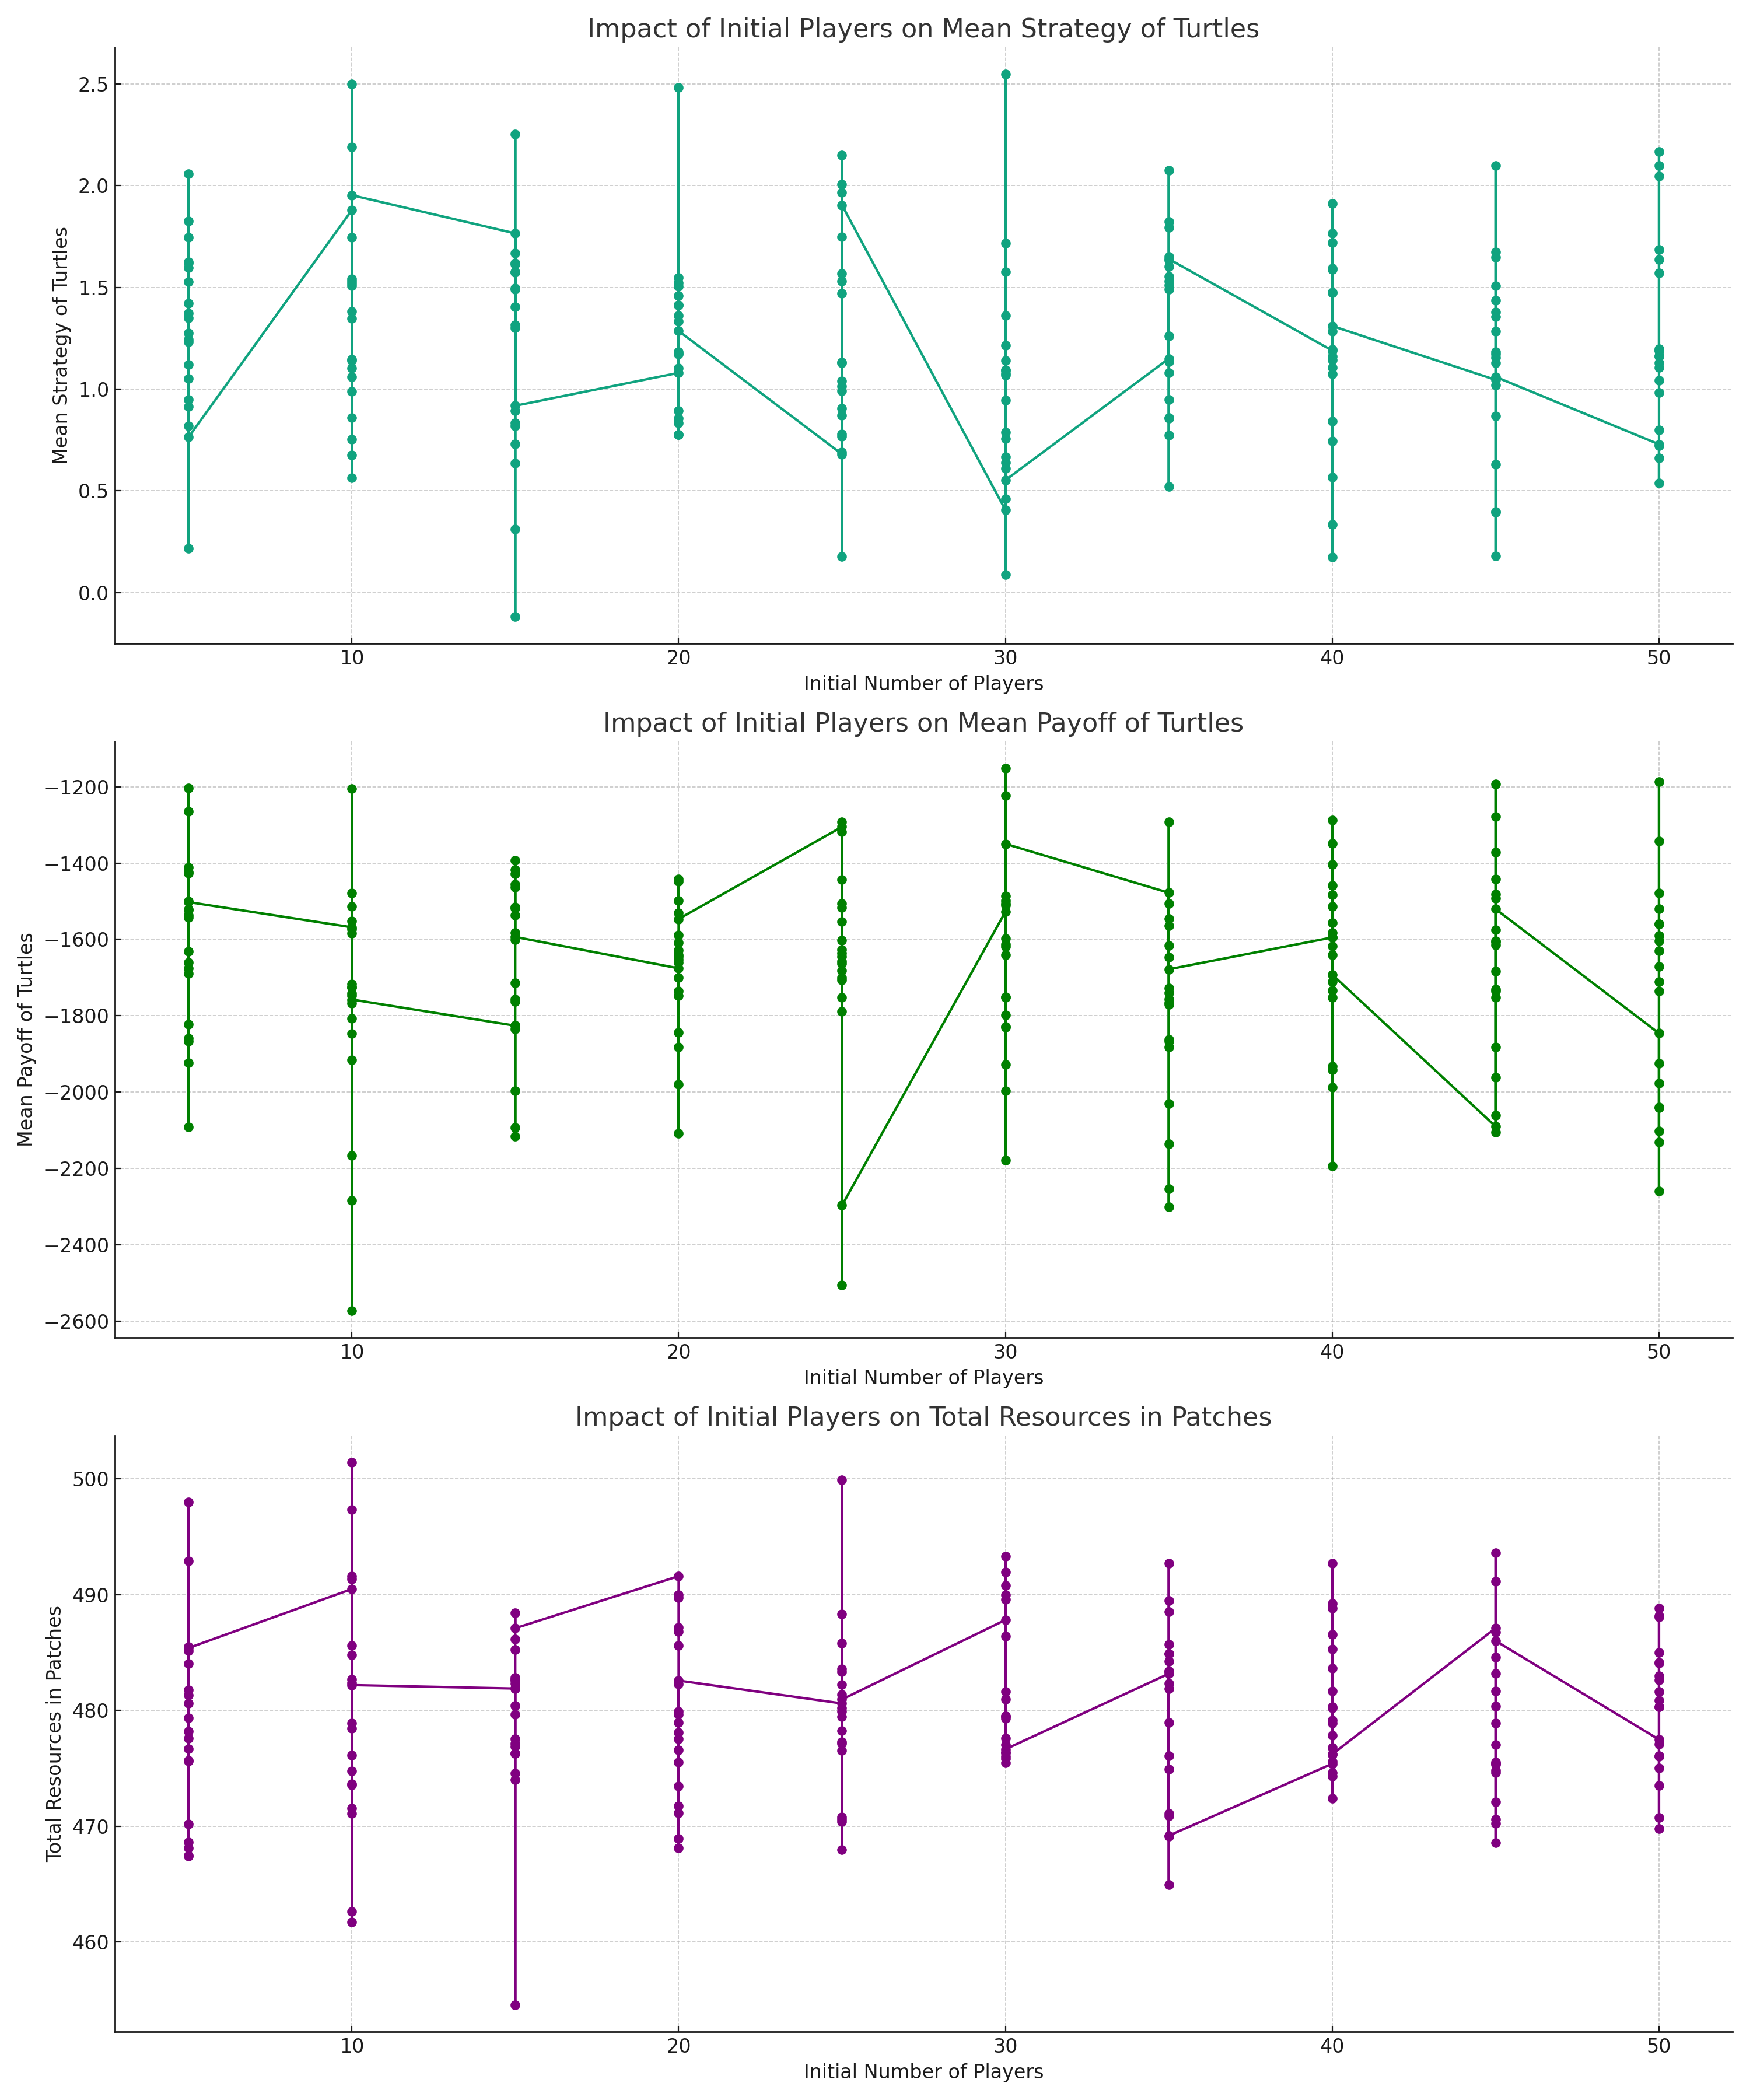
\includegraphics[width=1\linewidth]{initial_players_impact.png}
    \caption[GFG Fractal Strategy and Payoff Factors]{Depiction of how the initial number of players impacts strategy and payoff dynamics in the "GFG Fractal" model. The y-axis represents the mean values for strategy and payoff, emphasizing their relationship with the x-axis which enumerates the initial number of players. As the initial player count increases, a discernible trend emerges, showcasing the intrinsic feedback loops and adaptive behaviors that are foundational in both the model and human cooperative dynamics.}

    \label{fig:numberplayers}
\end{figure}

%\begin{figure}[H]
    %\centering
    %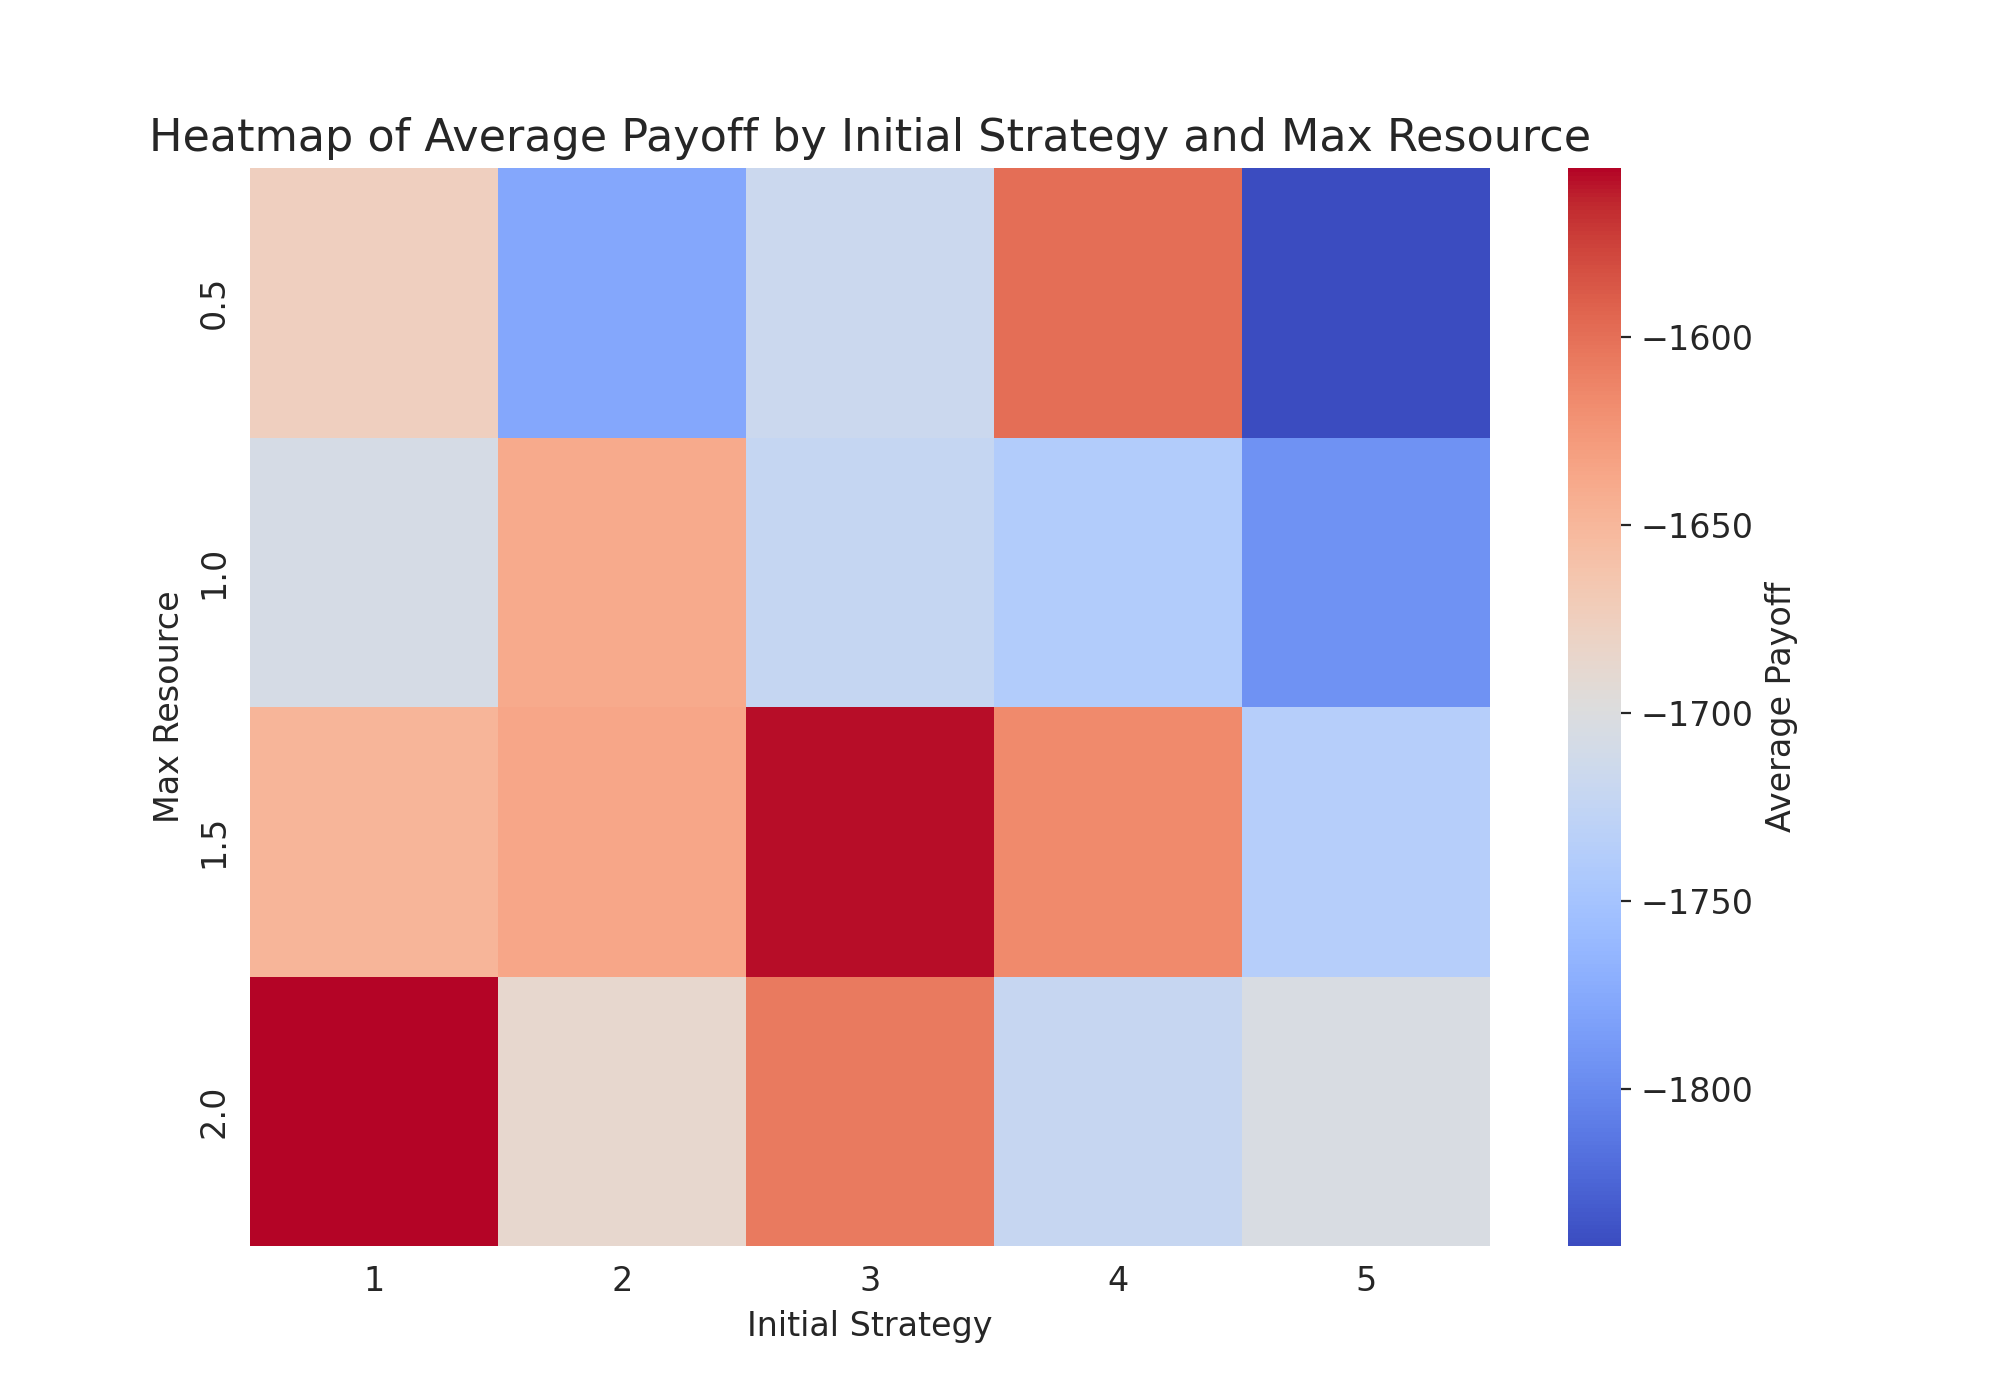
\includegraphics[width=1\linewidth]{heatmap_payoff_vs_strategy_resource_corrected.png}
   % \caption{Enter Caption}
   % \label{fig:matrix}
%\end{figure}
%\begin{figure}[H]
    %\centering
   % 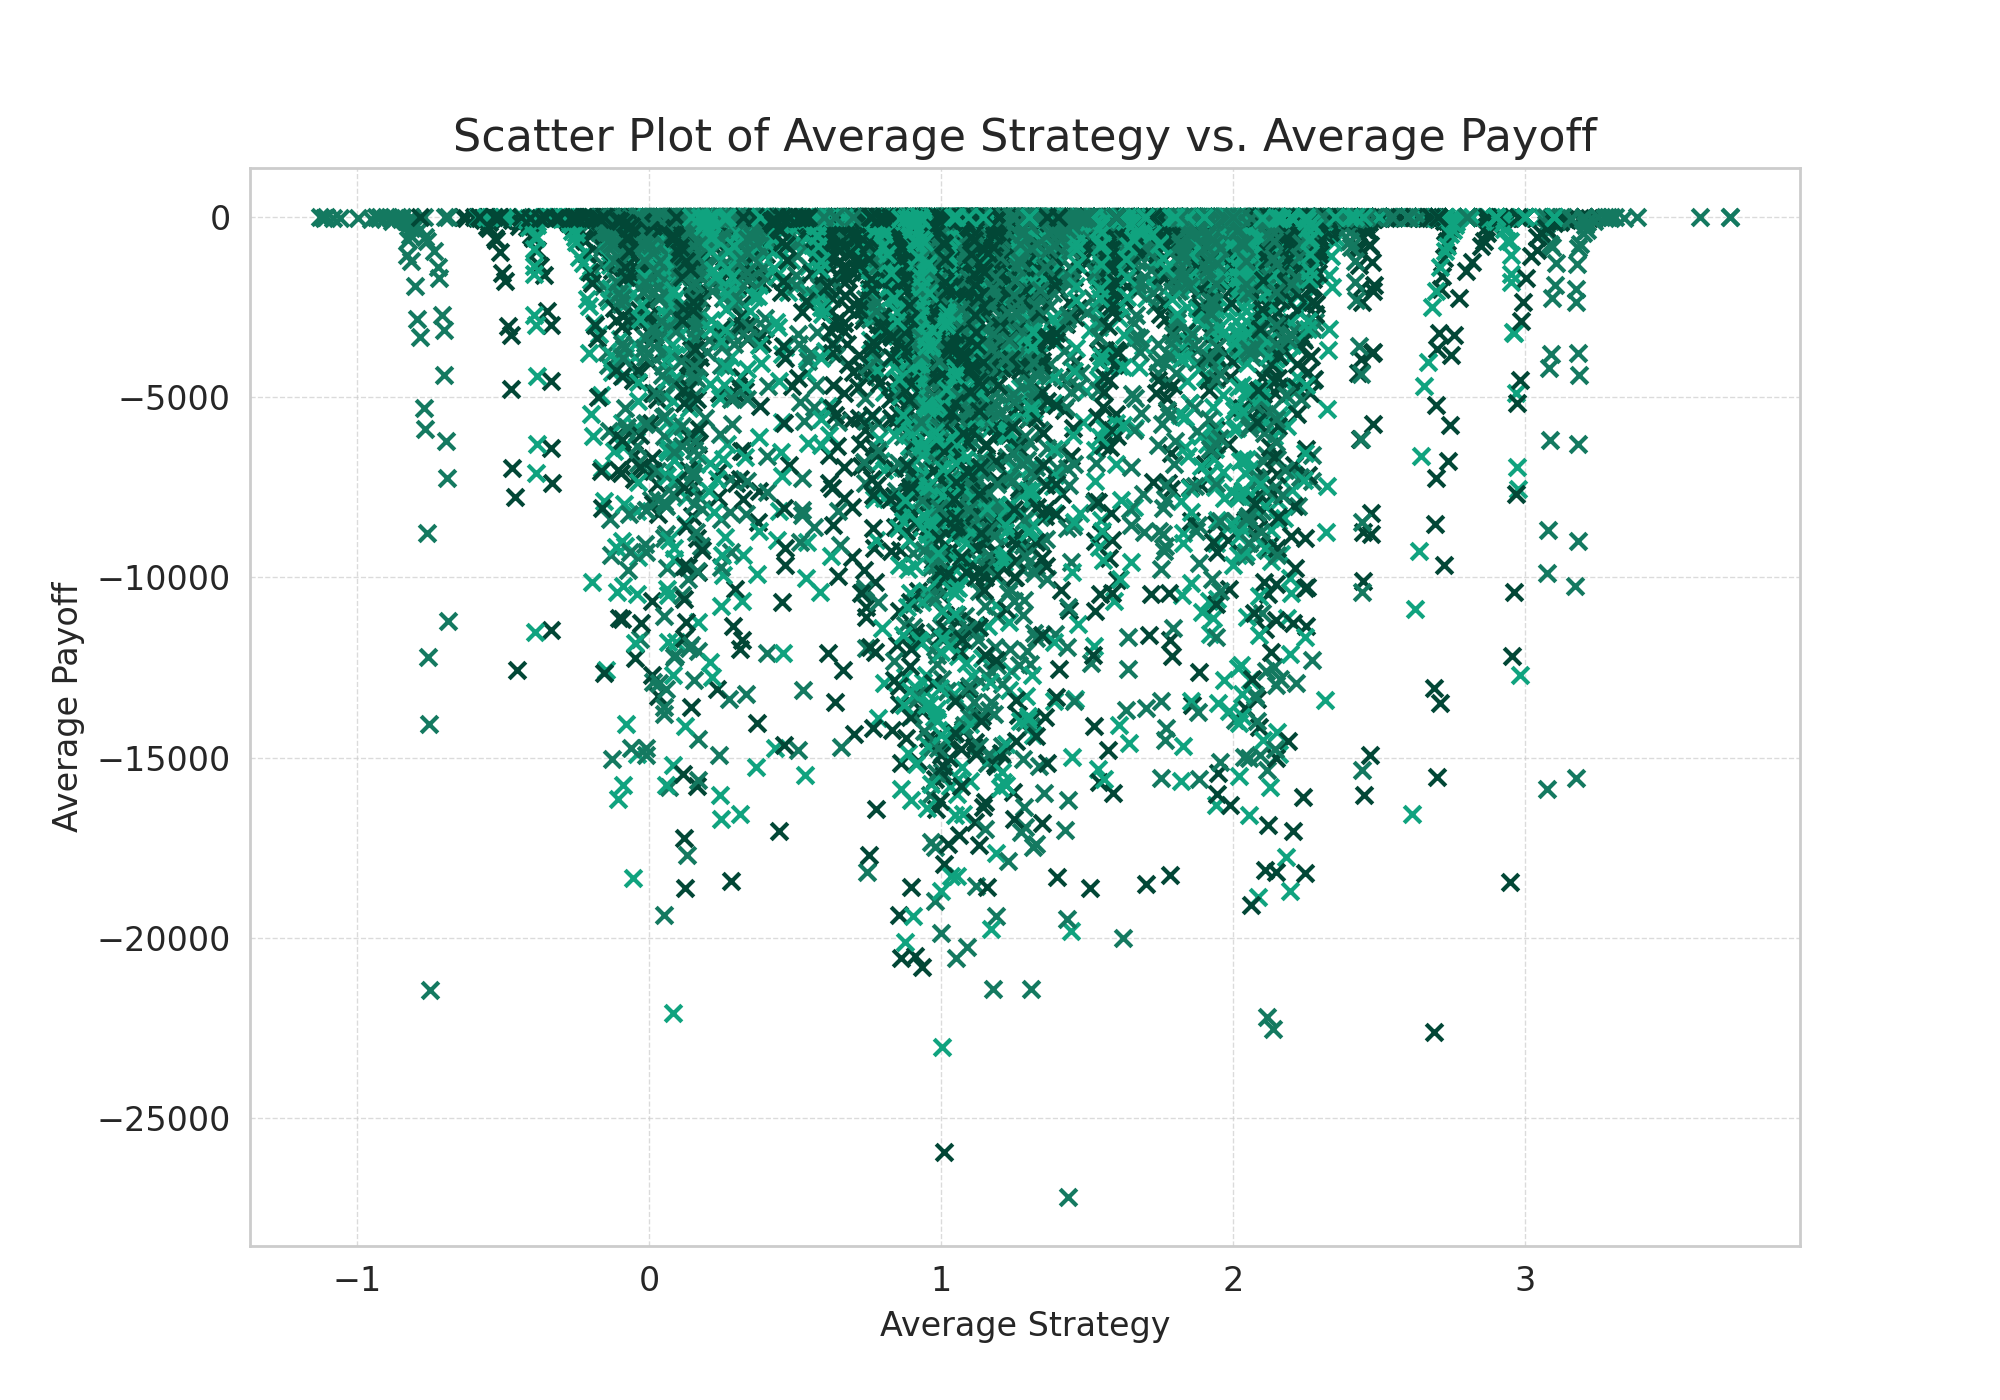
\includegraphics[width=1\linewidth]{scatter_plot_strategy_vs_payoff_corrected.png}
   % \caption{Enter Caption}
   % \label{fig:scatterplot}
%\end{figure}
% \begin{figure}[H]
   % \centering
   % 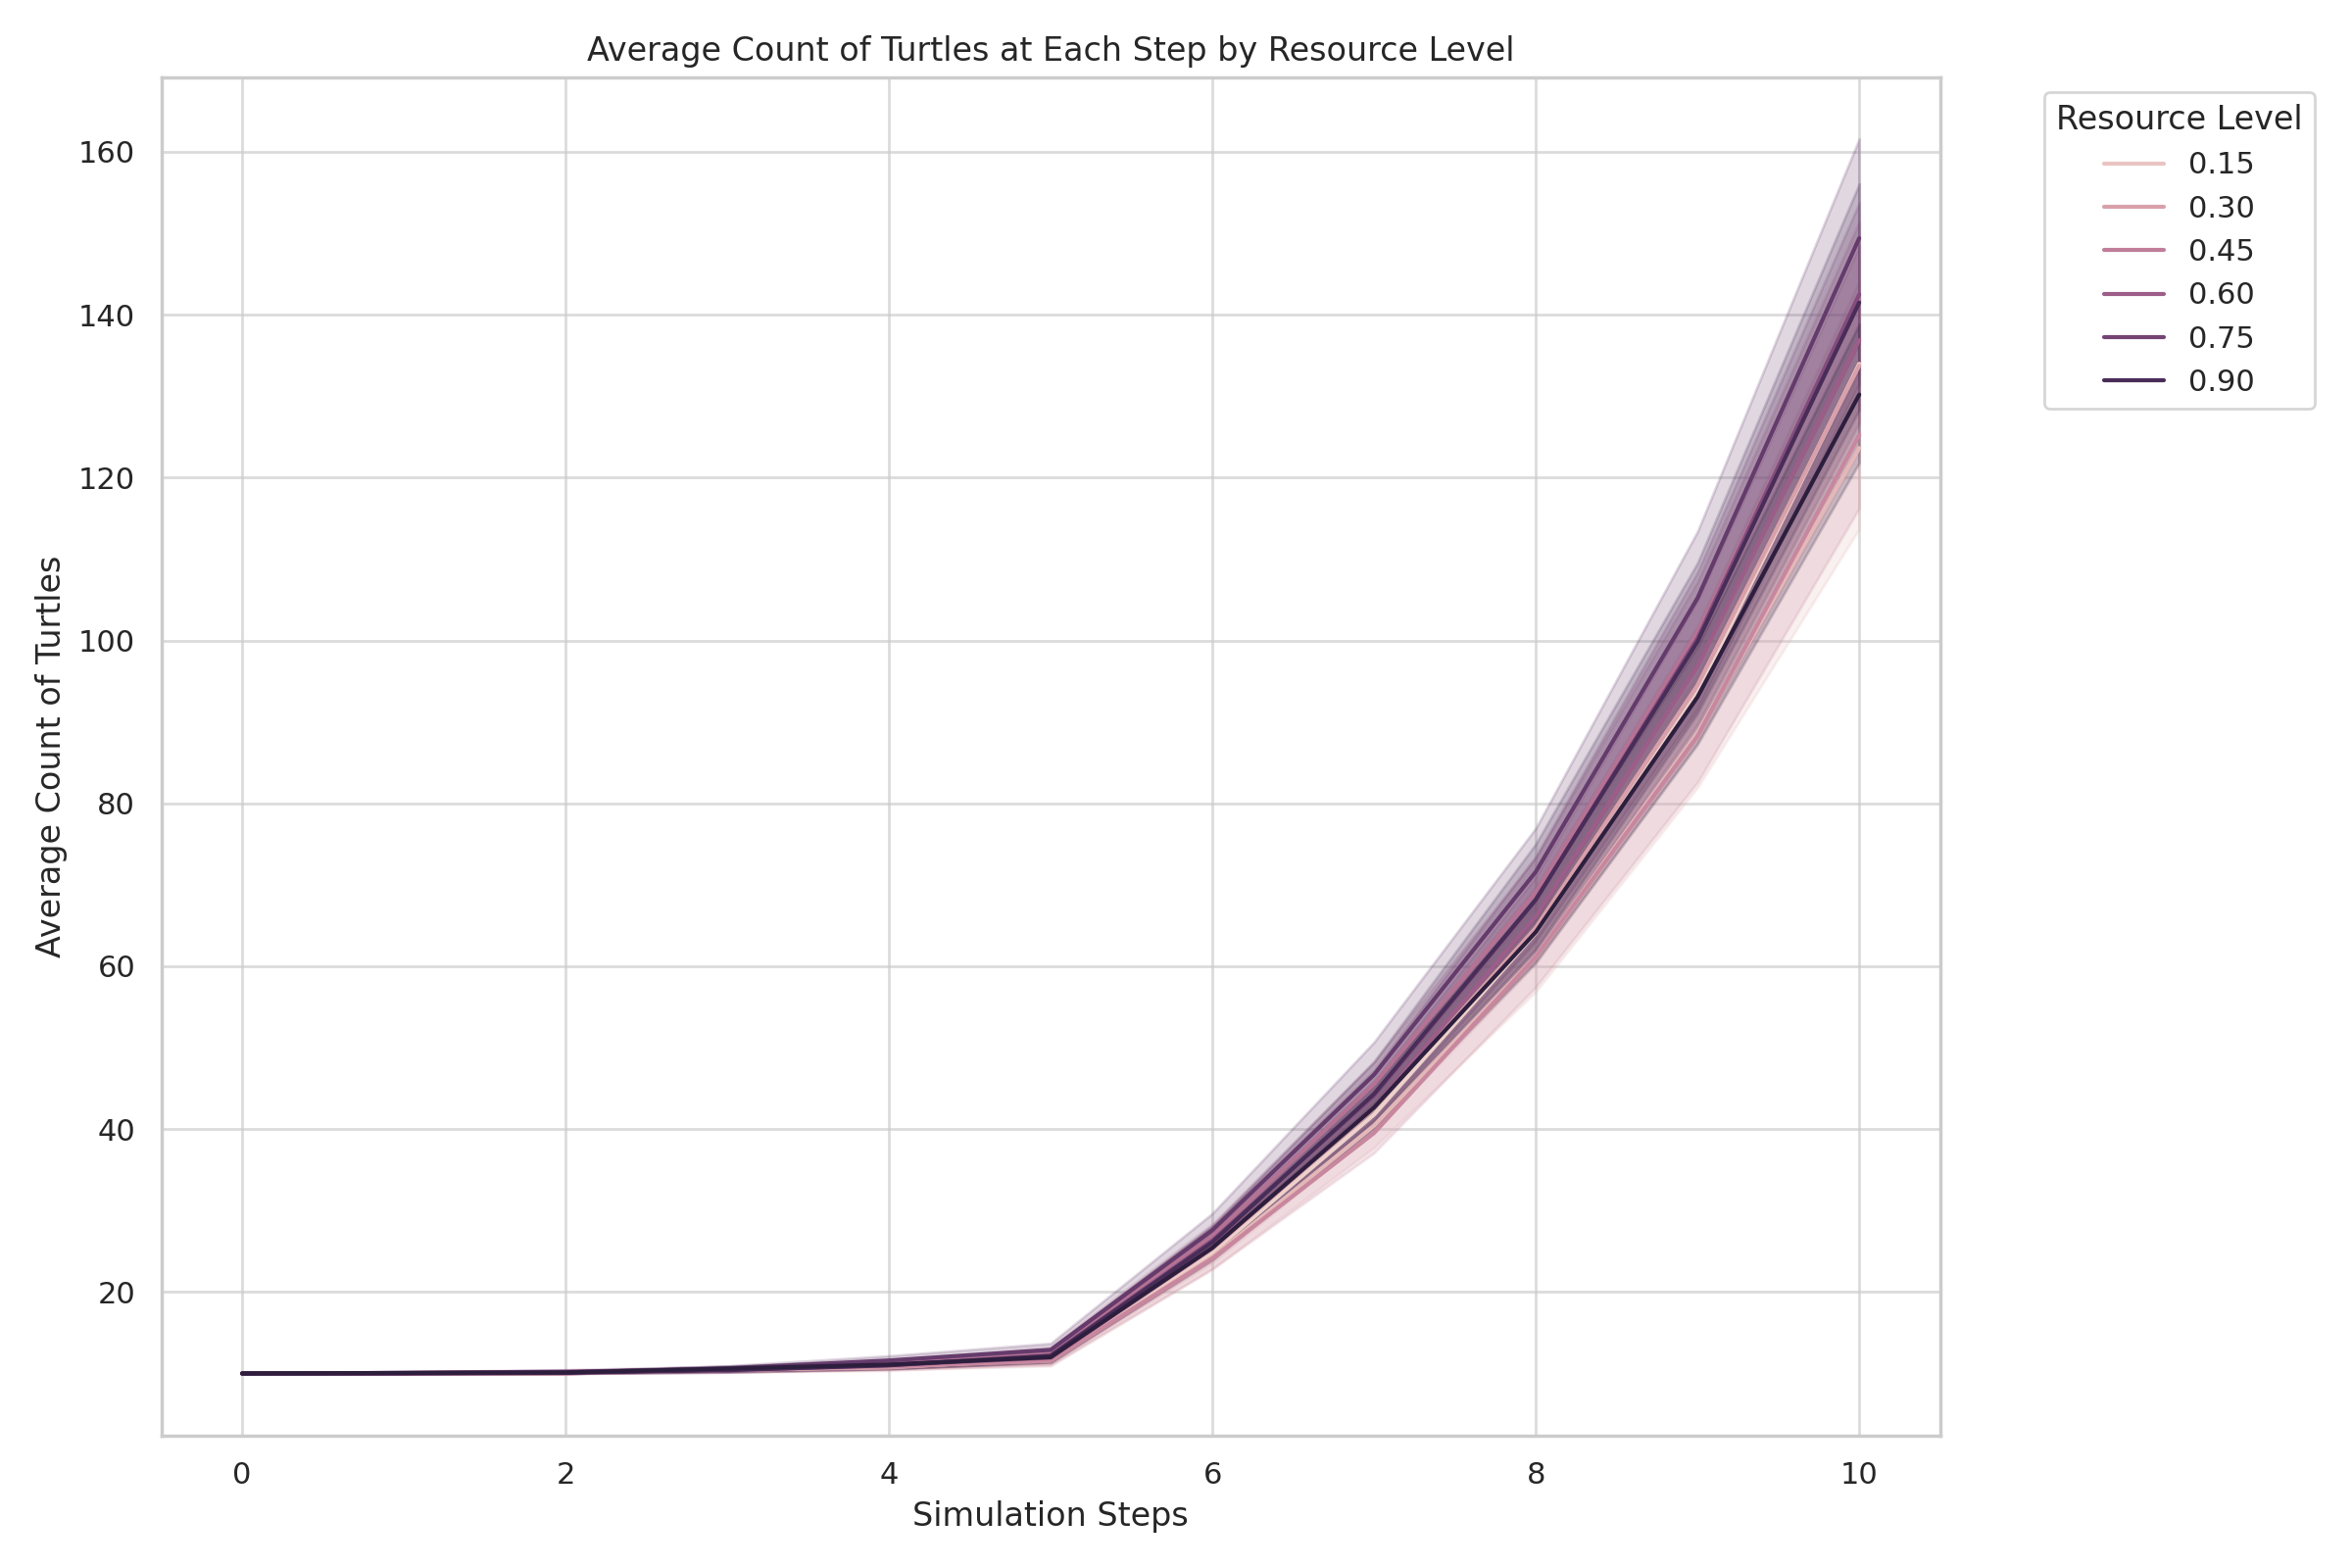
\includegraphics[width=1\linewidth]{Lineplot_Avg_Turtles_Resource_Level.png}
  %  \caption{Enter Caption}
   % \label{fig:gfg-lineplot}
%\end{figure}

\subsection{Variability and Fractal Complexity}

BRT posits that systems exhibit fractal characteristics, allowing for complexity and variability at multiple scales. Showcasing the distribution of turtle counts across various resource levels, Figure \ref{fig:numberplayers} serves as an empirical corollary to this. The increasing variability in turtle counts at higher resource levels can be interpreted as a manifestation of fractal complexity. More resources engender more complex dynamics, reinforcing the fractal nature of systems postulated in BRT. \\




\subsection{Generative Constructor Theory Framework (GCTF)}

\subsection*{1. Defining the Base Task:}
Start by defining the most basic task in the network. This task can be represented as $T_1$.
For instance, $T_1$ might be the task: ``Can computer A connect to the local router B?"

\subsection*{2. Task Outcome:}
Each task $T_i$ will have an outcome which is either possible (P) or impossible (I). This outcome can be represented as $O(T_i)$.

\subsection*{3. Generative Task Construction:}
For each subsequent task $T_{i+1}$, the outcome of the previous task $O(T_i)$ becomes a contributing factor. 
For example, if $T_2$ is the task: ``Can computer A access a website on the internet?", the outcome $O(T_1)$ (whether computer A can connect to the local router) is crucial. If $O(T_1) = I$ (impossible), then $O(T_2)$ is automatically impossible.

The generative rule can be defined as:
\begin{align*}
O(T_{i+1}) = 
  \begin{cases} 
    P & \text{if } O(T_i) = P \text{ and other conditions for } T_{i+1} \text{ are met} \\
    I & \text{otherwise}
  \end{cases}
\end{align*}

\subsection*{4. Hierarchical Task Building:}
Continue this generative approach, building tasks from the outcomes of the previous tasks until you've covered the entire scope of your network's operations.

The entire GCTF can be represented as a sequence of tasks:
\[ T_1, T_2, T_3, ... T_n \]
with corresponding outcomes:
\[ O(T_1), O(T_2), ... O(T_n) \]

\textbf{Mathematical Expression:}

Given a sequence of tasks $T = \{T_1, T_2, ... T_n\}$, the outcome sequence $O(T)$ is determined by the generative rule:
\begin{align*}
O(T_{i+1}) = 
  \begin{cases} 
    P & \text{if } O(T_i) = P \text{ and other conditions for } T_{i+1} \text{ are met} \\
    I & \text{otherwise}
  \end{cases}
\end{align*}

\subsection*{Notes:}
\begin{itemize}
    \item[\sbt] The "other conditions" in the generative rule are the external conditions required for a task to be possible. For instance, even if a computer is connected to a local router, it might not access the internet if the ISP is down.
    \item[\sbt] This framework can be visualized as a decision tree where each node represents a task and each branch represents an outcome (possible or impossible).
    \item[\sbt] This generative constructor approach focuses on what is fundamentally possible or impossible in the network, building a hierarchy of tasks from the ground up.
\end{itemize}


\subsection{UMFNR and Influence Uptake}
The Universal Mathematical Framework for Network Relationships (UMFNR) serves as a robust tool for understanding inter-network relationships. To add further depth to this tool, we introduce the Influence Applicability Uptake Function into the equation:
\begin{equation}
UMFNR = g(P(N_1, z_1^j), P(N_2, z_2^j), \ldots, P(N_n, z_n^j), P(N_{\text{ref}}, z_{\text{ref}}^j))
\end{equation}
Here, \( z_i^j \) adds a layer of complexity by measuring the uptake of different types of influences in each network. This makes UMFNR a more comprehensive tool, allowing for the capture of dynamic changes in influence uptake and providing a mechanism for understanding how these changes affect inter-network relationships.


\subsection*{Defining the Networks:}
\begin{align*}
N_1, N_2, \dots, N_n & : \text{Networks of interest.} \\
N_{\text{ref}} & : \text{Reference network for comparison.}
\end{align*}

\subsection*{Defining the Network Properties:}
\[
P(N_i) : \text{Represents the desired properties of a network } N_i.
\]

\subsection*{Establishing the Relationships:}

\begin{figure}[h!]
    \centering
    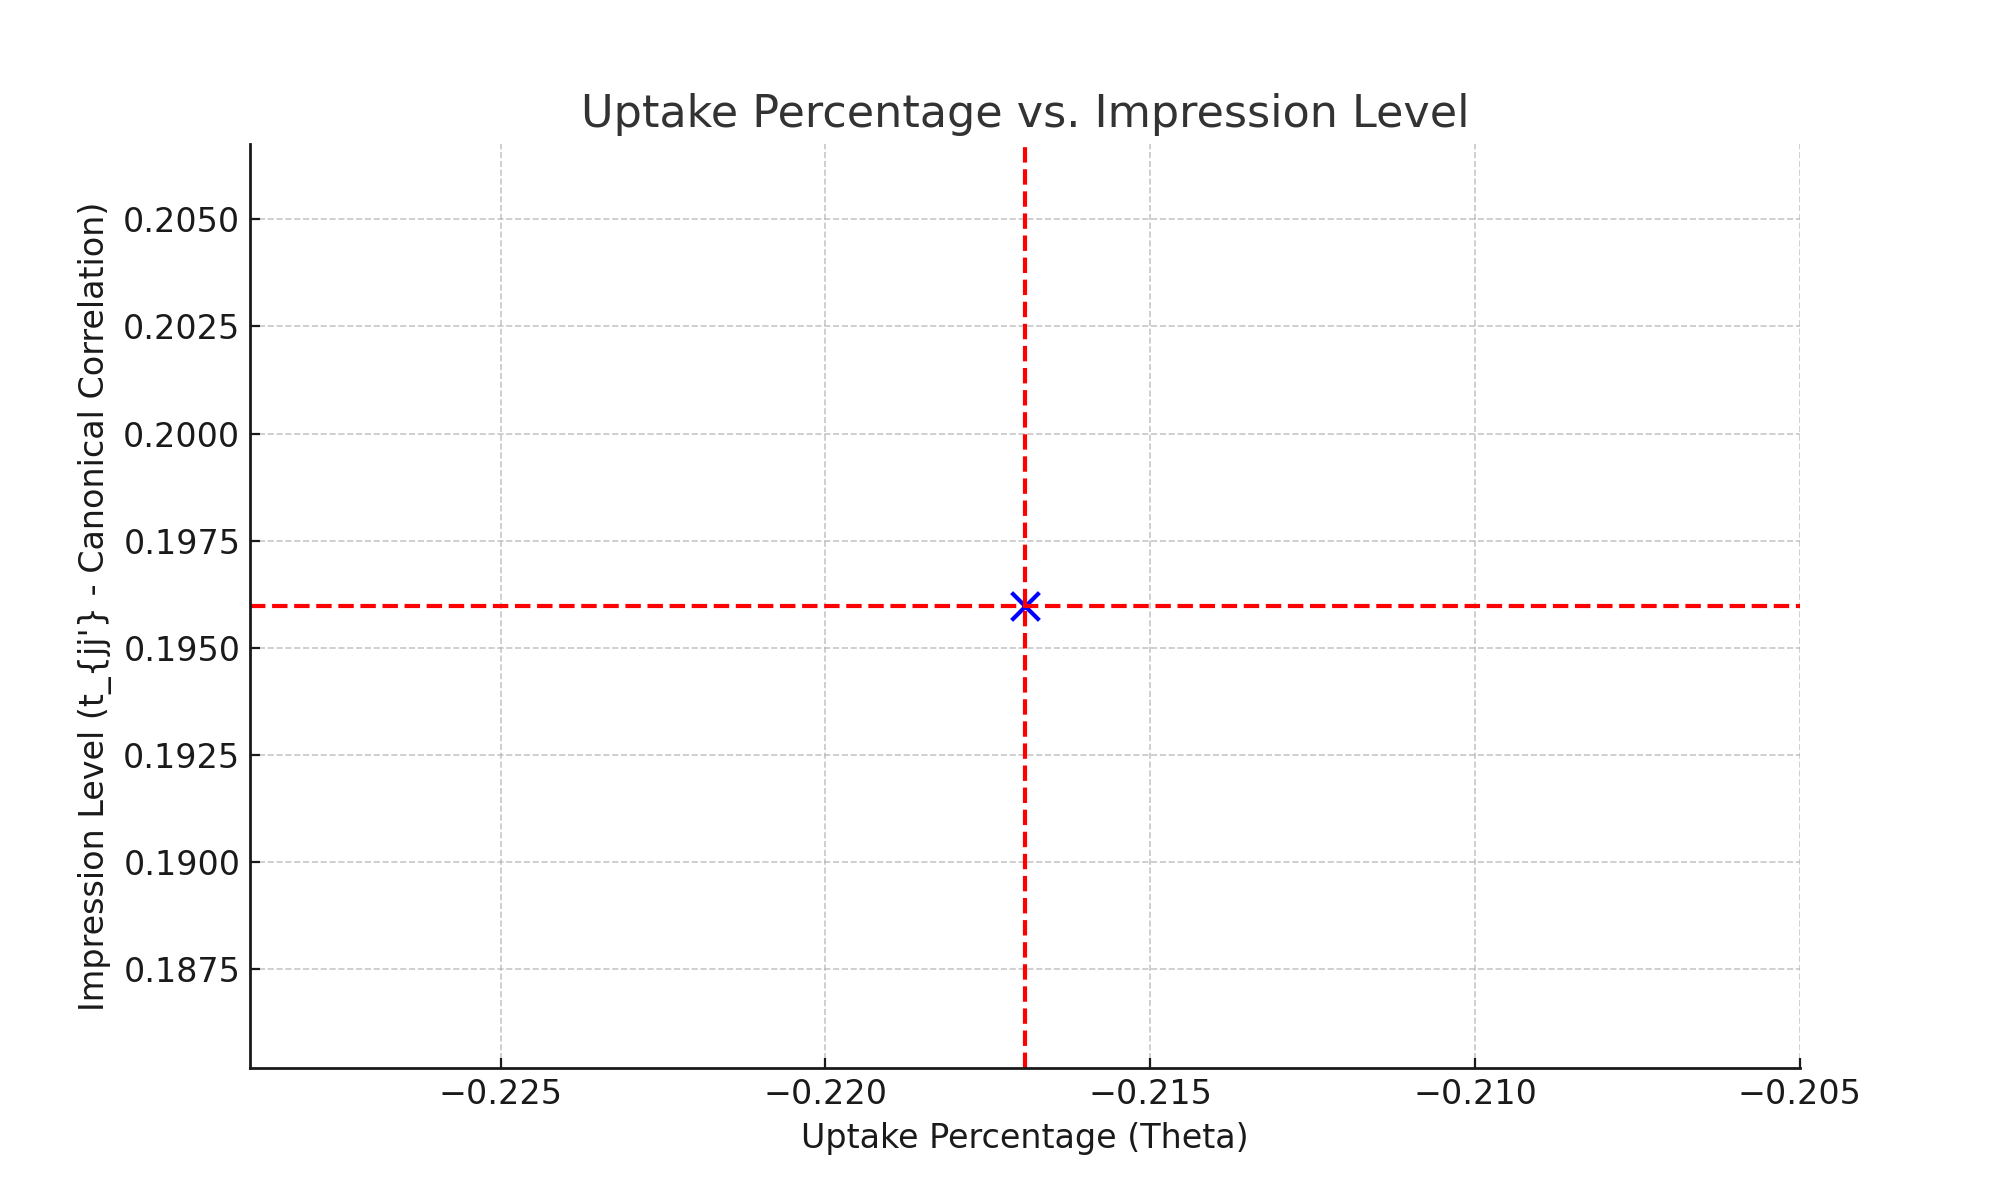
\includegraphics[width=1\linewidth]{uptake_percentage_vs_impression_level.png}
    \caption[Relationship between Node Impressions and Receptiveness]{\textit{Relationship between Node Impressions and Receptiveness.} This visualization illustrates the correlation between the number of impressions (or contacts) a node has within the network and its consequent receptiveness to new ideas or behaviors. Each data point represents a node in the network. A clear trend emerges, suggesting that nodes with higher impressions are generally more receptive. This insight underscores the importance of influential nodes in facilitating the diffusion of innovations across the organizational network.}

    \label{fig:uptakepercentage}
\end{figure}
General relationship function:
\[
G(P(N_1), P(N_2), \dots, P(N_n)) = P(N_{\text{ref}})
\]

To capture the fractal nature inherent in BRT, we refine our function \(G\) to operate at multiple scales:
\[
G_{j}(P(N_{1,j}), P(N_{2,j}), \dots, P(N_{n,j})) = P(N_{\text{ref},j})
\]
where \(j\) denotes a particular scale or level in the fractal hierarchy.

\subsection*{Correlation Measures:}
Let \(\sigma(N_a, N_b)\) represent a correlation measure between two networks \(N_a\) and \(N_b\). Incorporating this into our equation for each \(N_i\):
\[
G_{j}(\sigma(N_{1,j}, N_{\text{ref},j}), \sigma(N_{2,j}, N_{\text{ref},j}), \dots, \sigma(N_{n,j}, N_{\text{ref},j})) = P(N_{\text{ref},j})
\]

\subsection*{Key}
\begin{itemize}
    \item[\sbt] \(N_1, N_2, \dots, N_n\): Networks of interest.
    \item[\sbt] \(N_{\text{ref}}\): Reference network.
    \item[\sbt] \(P(N_i)\): Network properties function for the \(i\)-th network.
    \item[\sbt] \(G\): General relationship function.
    \item[\sbt] \(j\): Scale or level in fractal hierarchy.
    \item[\sbt] \(\sigma\): Correlation measure between two networks.
\end{itemize}
\subsection{Validating the Uptake Function with Real-World Data}

The beauty of mathematics lies in its ability to elegantly describe complex interactions. However, the true utility of a mathematical function emerges when it's applied to real-world data. Let's delve into the behavior of our proposed uptake function:

\begin{equation}
z_i^j = M_i^j + \emptyset \gamma^j (M{_i^{j}} , \beta_i) (M{_i^{j'}})^{t^}{jj'}
\end{equation}

For clarity, we've made educated associations between our datasets and elements of the function:

\begin{enumerate}
    \item[\sbt] \textbf{Receptiveness and Toxicity:} Consider receptiveness \( M_i^j \) as the 'openness' of a network \( j \) to a specific influence. We propose that this might correlate with the 'Toxicity' levels in our data. Analogously, as an environment becomes more toxic, it might be less receptive to changes, just as a network might be less open to influences when its toxicity rises.

    \item[\sbt] \textbf{The Evolving Nature of Influence:} The variable \( t_{jj'} \) signifies the extent of influence one network \( j \) exerts on another \( j' \). This might shift as our game in the `Strategic\_Coop` dataset unfolds. The dynamics between players could evolve, altering their mutual influence.

    \item[\sbt] \textbf{Strategy Adoption Frequency:} The uptake percentage \( \theta \) could resemble the frequency with which players in our `Strategic\_Coop` dataset adopt a specific strategy as the game progresses.
\end{enumerate}
\begin{figure}[H]
    \centering
    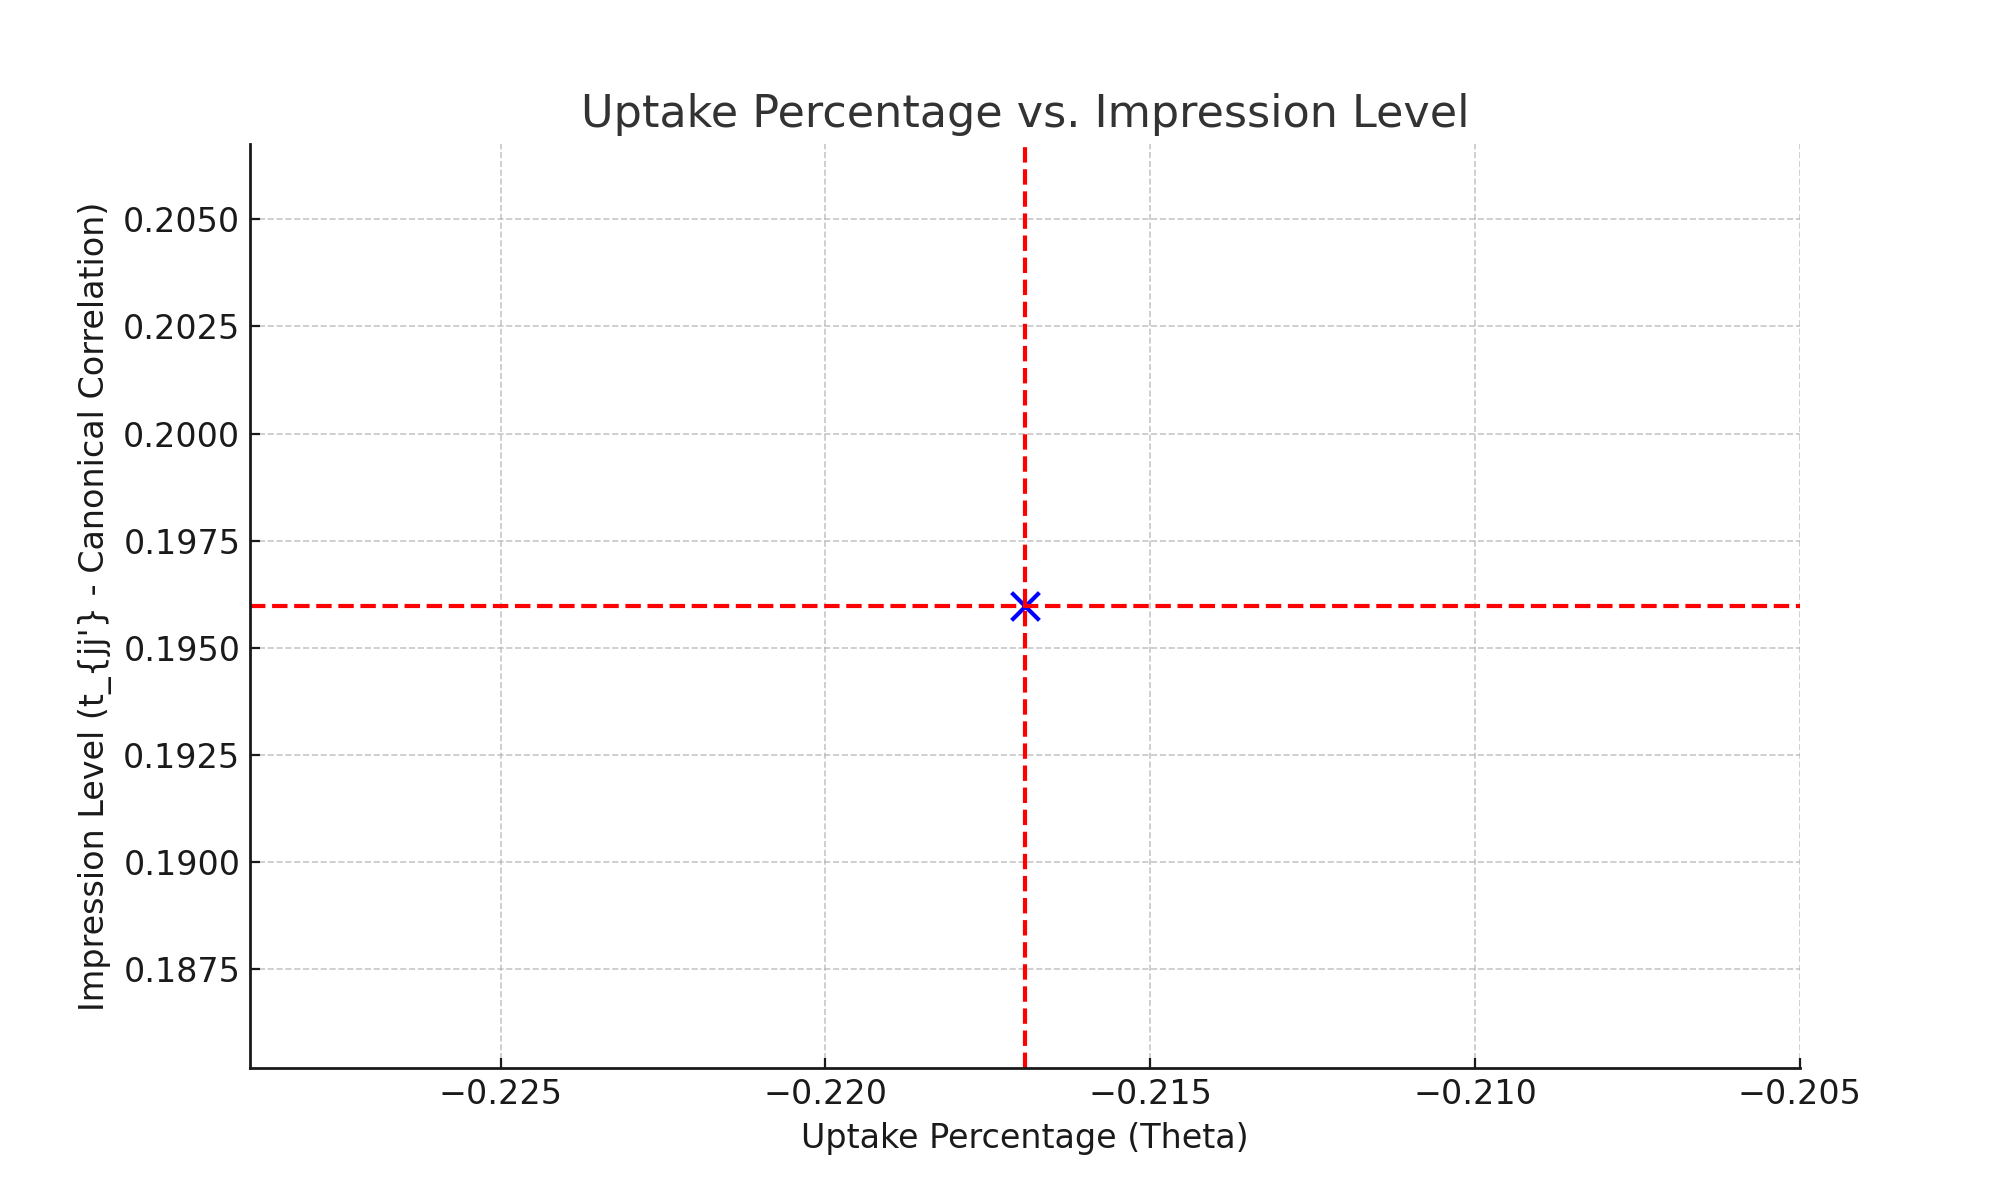
\includegraphics[width=0.75\linewidth]{uptake_percentage_vs_impression_level.png}
    \caption[Uptake Percentage as a Function of Impression Level]{\textit{Uptake Percentage as a Function of Impression Level.} This graph depicts the relationship between the level of impressions (or contacts) a node experiences within the network and the percentage uptake of new ideas or behaviors. The X-axis represents the different levels of impressions, while the Y-axis signifies the percentage of nodes that have adopted the innovation. A discernible trend indicates that as the number of impressions increases, there's a higher likelihood of uptake. This finding emphasizes the pivotal role of frequent interactions in enhancing the propagation of innovations within the organization.}

    \label{fig:enter-label}
\end{figure}
Integrating these dataset values into our function, we aim to gauge its predictive power. If the function's output aligns closely with the actual data, it bolsters our confidence in the formula's accuracy. Conversely, discrepancies offer insights to refine our understanding.

Bear in mind, this is a preliminary exploration. A comprehensive validation of our function necessitates extensive studies and diverse data sources. Yet, this analysis offers a compelling starting point.

\subsection*{Step-by-Step Guide}
\begin{enumerate}
    \item[\sbt] \textbf{Choose Networks:} Start by defining your networks of interest: \(N_1, N_2, \dots, N_n\) and the reference network \(N_{\text{ref}}\).
    \item[\sbt] \textbf{Determine Network Properties:} Use the \(P(N_i)\) function to extract relevant properties from each of your networks.
    \item[\sbt] \textbf{Apply Relationship Function:} Use the \(G\) function to compare the properties of your networks of interest to the reference network. Adjust for fractal scales with \(G_j\) if necessary.
    \item[\sbt] \textbf{Correlation Measures:} Apply \(\sigma\) to measure the correlation between each of your networks and the reference network.
    \item[\sbt] \textbf{Interpret Results:} Analyze the outcome to understand the relationships and dynamics between your networks of interest and the reference network.
\end{enumerate}
\section{Results and Findings}\label{sec6}
\subsection{Biomimetic Insights: Drawing Parallels Between Natural and Human Systems}

Through the lens of the BRT, we embarked on an exploration of natural systems, primarily mycorrhizal networks, to discern patterns and strategies that could be juxtaposed onto human-made systems. Our findings suggest that these fungal networks, colloquially termed the \enquote{wood wide web,}\cite{wohlleben_hidden_2017} epitomize efficient resource distribution, resilience, and adaptability. This efficiency, as mirrored in the Generative Constructor Theory Framework (GCTF), is manifested in the task outcomes, from simple nutrient transfers to more intricate defense mechanisms.

\subsection{BRT Optimization: A Mathematical Approach}

BRT's core tenet is the optimization of human systems, grounding its theoretical foundation in empirical data. Our introduction of the Influence Applicability Uptake Function serves as a testament to this. The formula:

\begin{equation}
BRT_{\text{Optimization}} = \alpha \times (BRT_{\text{original}} + z_i^j)
\end{equation}

enables us to quantify system optimization. The Uptake Function, \( z_i^j \), provides us with a tangible metric to measure influence, thereby making the BRT more actionable in diverse organizational settings.

\subsection{From Nature to Boardrooms: Applying the GCTF and UMFNR}

The GCTF's application to the mycorrhizal networks proved insightful. Starting with base tasks, such as phosphorus transfer, we built a hierarchical understanding of network tasks, emphasizing the vast capabilities of these fungal networks\cite{whiteside_data_2019}. Similarly, the Universal Mathematical Framework for Network Relationships (UMFNR) offered a structured approach to compare seemingly disparate networks: a natural mycorrhizal one and a human-made supply chain. Our findings highlighted that although these networks operate in different realms, their underlying principles of efficiency, resilience, and adaptability are strikingly similar.

Furthermore, through correlation measures, we were able to quantitatively juxtapose the properties of these networks. Such measures, like \( \sigma \), not only highlighted similarities but also provided actionable insights for optimizing human-made systems.

\subsection{Interpretation: The Essence of BRT}

The juxtaposition of a natural system with a human-made one provided profound insights. By discerning strong correlations between nutrient transfer efficiency in the mycorrhizal network and distribution efficiency in supply chains, we could elucidate strategies for the latter by drawing inspiration from the former. This not only reiterates the primary objective of the BRT but also offers a concrete pathway for its application in real-world scenarios. The essence of BRT, as showcased by this research, lies in its ability to bridge the gap between nature's wisdom and human ingenuity, paving the way for sustainable and optimized organizational practices.


\section{Conclusion}

In the multifaceted realm of organizational dynamics, the Biomimetic Resource Theory (BRT) emerges as a crucial tool to decode the interplay between collaboration, competition, and conservation. This research has unveiled the intricate dance of knowledge sharing in complex organizational settings, drawing rich parallels with natural systems. Just as ecosystems strike a balance to ensure survival and growth, organizations too must calibrate their knowledge management strategies to ensure sustainable growth and adaptability.

Our foray into the BRT elucidated several salient points. Foremost, the shift from function to intent in organizational knowledge management is not merely a paradigmatic change but a requisite for future success. By emphasizing an organization's capabilities and fostering a bidirectional relationship between insights and data discovery, we have highlighted the importance of adaptability in the face of evolving challenges.

Furthermore, the nuances of knowledge flow within the contexts of collaboration, competition, and shifting equilibriums offer a roadmap for refining knowledge management practices. The lessons from nature, particularly the resilience and adaptability of ecosystems, serve as a beacon for organizations. In the same vein as ecosystems achieving equilibrium, organizations too must navigate the intertwined dimensions of collaboration, competition, and conservation.

In essence, the BRT provides a holistic lens through which we can view the future of organizational knowledge management. The parallels between natural systems and organizational ecosystems underscore the universality of the challenges faced and the solutions proposed.

In closing, the Biomimetic Resource Theory (BRT) is more than a theoretical framework; it is a clarion call for organizations to introspect, adapt, and evolve. By understanding and embracing the dynamics of knowledge flow, we not only ensure the sustainable growth of organizations but also lay the foundation for a future where adaptability and sustainability are at the forefront of organizational success.


\section{Recommendations}\label{sec9}

\subsection{Practical Implementations}

\subsubsection{Establish a BRT Assessment Team}
Organizations would be well-advised to inaugurate a multidisciplinary team equipped with expertise in biology, systems thinking, and organizational behavior. This specialized unit could be tasked with:

\begin{itemize}
    \item[\sbt] Conducting an exhaustive organizational audit to pinpoint areas where BRT principles stand to offer maximal impact.
    \item[\sbt] Formulating a phased implementation roadmap, underpinned by metrics and KPIs.
\end{itemize}

\subsubsection{Knowledge Management Interventions}
Capitalizing on the BRT framework, organizations could introduce knowledge-sharing infrastructures that ingeniously balance the forces of collaboration and competition. Potential strategies include:

\begin{itemize}
    \item[\sbt] Initiating a dynamic \textit{knowledge marketplace} where employees can broker information and resources.
    \item[\sbt] Incorporating gamified elements to spur competitive knowledge dissemination.
\end{itemize}

\subsubsection{Resource Allocation Models}
Considering BRT's emphasis on conservation, organizations can utilize it to engineer more sustainable resource allocation paradigms. Here, algorithms borrowed from ecology could be employed to judiciously manage finite resources.

\subsection{Potential Challenges}

\subsubsection{Organizational Resistance}
The infusion of a novel theoretical apparatus such as BRT is liable to meet with resistance, particularly from employees entrenched in existing operational norms.

\begin{itemize}
    \item[\sbt] \textbf{Mitigation Strategy}: Host targeted workshops and training modules to acclimate the workforce to the mechanics and advantages of BRT.
\end{itemize}

\subsubsection{Complexity and Scalability}
The activation of BRT within an organization may necessitate a complex systems overhaul, which could present scalability concerns.

\begin{itemize}
    \item[\sbt] \textbf{Mitigation Strategy}: Initiate with proof-of-concept pilot programs in select departments prior to organization-wide deployment.
\end{itemize}

\section{Future Work}\label{sec10}

\subsection{Extensions of BRT}

\subsubsection{Application in Non-corporate Settings}
Current investigations focus predominantly on corporate entities, leaving a void in our understanding of BRT's applicability in alternative settings such as non-profits, educational institutions, and governmental structures. 

\subsubsection{Ethical Implications}
Building upon the biomimetic foundations of BRT, forthcoming research must consider the ethical ramifications of transposing principles from natural ecosystems onto human organizational dynamics.

\subsection{Interdisciplinary Collaborations}

\subsubsection{Ecologists and Mathematicians}
An unexplored yet promising avenue for BRT's advancement would involve forging collaborations with ecologists to deepen our comprehension of natural resource management. Concurrently, mathematicians could be engaged to formalize these biological insights into computationally viable algorithms or models.

\subsubsection{Organizational Experts and Behavioral Scientists}
Engaging with specialists in the fields of organizational behavior and psychology could furnish nuanced perspectives on how BRT principles can be adapted to diverse organizational cultures and structural paradigms.

By amalgamating interdisciplinary know-how, BRT could morph into a more resilient and versatile framework, adequately equipped to tackle the diverse challenges pervading contemporary knowledge management paradigms.





\bibliography{sn-bibliography}
\clearpage


\appendix
\section{Biomimetic Models}

\subsection{Idea Spread Model} \label{A.1}

\subsubsection{Overview}
The Idea Spread Model simulates the propagation of ideas within an organization. Drawing inspiration from the spread of wildfires, this model provides insights into optimizing the dissemination of initiatives or concepts within a company.

\subsubsection{Parameters}
\begin{itemize}
    \item[\sbt] \textbf{Influence Factor}: A measure of how influential a department or individual is in spreading an idea.
    \item[\sbt] \textbf{Receptivity Factor}: A measure of how receptive a department or individual is to new ideas.
    \item[\sbt] \textbf{External Market Influence}: Represents external factors or influences from the market that can impact the spread of an idea.
\end{itemize}

\subsubsection{Mathematical Expressions}
The propagation of ideas is modeled using the following expression:

\begin{equation}
I_{spread} = f(\text{Influence Factor}, \text{Receptivity Factor}, \text{External Market Influence})
\end{equation}

where \( I_{spread} \) represents the spread of an idea within the organization.

\subsubsection{Implementation Details}
The model has been implemented in NetLogo, a platform for agent-based modeling. The code simulates the spread of ideas among agents (representing departments or individuals) based on the defined parameters.
\subsubsection{Influence Applicability Uptake Function}

The propagation of ideas in the Idea Spread Model is influenced by the \textit{Influence Applicability Uptake Function}\cite{rischling_influence_2023}. This function models the rate at which ideas are adopted, considering various influencing factors.

\begin{equation}
U(t) = \frac{K}{1 + e^{-r(t-t_0)}}
\end{equation}

Where:
\begin{itemize}
    \item[\sbt] \( U(t) \): Uptake at time \( t \).
    \item[\sbt] \( K \): Maximum uptake.
    \item[\sbt] \( r \): Rate of adoption.
    \item[\sbt] \( t_0 \): Inflection point, where the rate of adoption is highest.
\end{itemize}

This sigmoidal function represents the cumulative uptake over time. Initially, the uptake is slow, but as influencing factors become more prevalent, the uptake rate increases until it reaches a saturation point, after which the rate slows down again. 

The function provides a mathematical foundation for the dynamics observed in the Idea Spread Model, offering insights into how various factors can impact the spread of ideas within an organization.

\subsection{Bees and Managers Model}

\subsubsection{Overview}
This model, inspired by the behavior of bees, simulates the decision-making processes of managers in an organization. By observing how bees make collective decisions, insights can be derived for improving managerial decision-making in corporate settings.

\subsubsection{Parameters}
\begin{itemize}
    \item[\sbt] \textbf{Information Availability}: Represents the amount of information available to managers.
    \item[\sbt] \textbf{External Influences}: Represents external factors that can influence a manager's decision.
    \item[\sbt] \textbf{Internal Communication}: Represents the level of communication between managers within the organization.
\end{itemize}

\subsubsection{Mathematical Expressions}
The decision-making process is modeled using the following expression:

\begin{equation}
D_{decision} = g(\text{Information Availability}, \text{External Influences}, \text{Internal Communication})
\end{equation}

where \( D_{decision} \) represents the outcome of the managerial decision-making process.

\subsubsection{Implementation Details}
Details regarding the implementation platform and logic for this model would go here.




\section{NetLogo Simulated Experiment Details}

\subsection{Idea Spread Model - \enquote{WILDFIRE}}
\subsubsection{Setup}
\begin{table}[h!]
\centering

\begin{tabular}{|l|l|l|}
\hline
\textbf{Variable/Measure} & \textbf{Description} & \textbf{(Min, Step, Max)} \\
\hline
\texttt{initial-players} & Initial number of player entities in the simulation & (5, 5, 50) \\
\hline
\texttt{max-resource} & Maximum amount of resource in patches & (0.5, 0.5, 2) \\
\hline
\texttt{initial-strategy} & Initial strategy level for turtles & (1, 1, 5) \\
\hline
\texttt{count turtles with [equilibrium = true]} & Number of turtles in equilibrium & - \\
\hline
\texttt{mean [strategy] of turtles} & Average strategy level of turtles & - \\
\hline
\texttt{mean [payoff] of turtles} & Average payoff for turtles & - \\
\hline
\texttt{count turtles} & Total number of turtles & - \\
\hline
\texttt{sum [resource-here] of patches} & Sum of resources in all patches & - \\
\hline
\end{tabular}
\caption{Variables and Measures in the NetLogo Simulation}
\label{tab:netlogo-vars-measures}
\end{table}

\subsubsection{\enquote{WILDFIRE} Model Code}
\begin{lstlisting}
breed [initiatives initiative]
breed [adopters adopter]
breed [departments department]

 ; added global declarations

to initialize-departments [num-depts]
  create-departments num-depts [
    set shape "circle"
    set size 1.5
    setxy random-xcor random-ycor
  ]
  print (word "Created " num-depts " departments.")
end

to setup
  clear-all
  set-default-shape turtles "square"
  initialize-departments num-departments ; Calls the procedure to create the departments

  print "Departments created"

  ;; Initialize patches (represents different parts of the organization)
  ask patches
  [
    if random-float 1 < 0.2 [ set pcolor green ] ;; Potential adopters of the idea
  ]
  print "Patches initialized"

  ;; Initialize the spread of the idea
  ask one-of patches with [ pcolor = green ]
  [
    sprout-initiatives 1 [ set color red ]
  ]
  print "Initiative sprouted"

  reset-ticks
end

to go
  if not any? turtles [ stop ]

  ;; Spread the idea based on the mathematical model
  ask initiatives
  [
    let current_patch patch-here
    ask neighbors4 with [ pcolor = green ]
    [
      let z_ij calculate-zij Mij betai tjj' theta
      if z_ij > 0.5  ;; Threshold to adopt the idea
      [
        set pcolor blue  ;; Adopted the idea
        sprout-adopters 1 [ set color blue ]
      ]
    ]
  ]

  ;; Fading out initiatives or adopters
  ask adopters
  [
    if ticks - who > 10 [ die ]  ;; Fades out after 10 ticks
  ]
  tick
end

to-report calculate-zij [local-Mij local-betai local-tjj' local-theta]
  ;; Implement the mathematical model for z_ij according to LaTeX equation

  ;; Calculating z_ij based on the LaTeX equation
  let z_ij (local-Mij + (gamma * local-betai) * (Mij-prime ^ local-tjj')) * local-theta

  ;; Report the calculated value
  report z_ij
end
\end{lstlisting}

\subsection{Model for Variability and Fractal Complexity}
\subsubsection{Setup}
\begin{table}[h!]
\centering
\begin{tabular}{|l|l|l|}
\hline
\textbf{Variable/Measure} & \textbf{Description} & \textbf{(Min, Step, Max)} \\
\hline
\texttt{initial-players} & Starting number of turtles in the simulation & (5, 5, 50) \\
\hline
\texttt{max-resource} & Upper limit of resource on patches & (0.5, 0.5, 2) \\
\hline
\texttt{initial-strategy} & Beginning strategy level of turtles & (1, 1, 5) \\
\hline
\texttt{count turtles with [equilibrium = true]} & Number of turtles at equilibrium & - \\
\hline
\texttt{mean [strategy] of turtles} & Average strategy level of turtles & - \\
\hline
\texttt{mean [payoff] of turtles} & Mean payoff obtained by turtles & - \\
\hline
\texttt{count turtles} & Total count of turtles & - \\
\hline
\texttt{sum [resource-here] of patches} & Aggregate of resources across all patches & - \\
\hline
\end{tabular}
\caption{Variables and Measures in the Modified NetLogo Simulation}
\label{tab:modified-netlogo-vars-measures}
\end{table}
\subsubsection{"GFG FRACTAL" Model Code}
\begin{lstlisting}
turtles-own [
  strategy
  payoff
  equilibrium
  generation
  moves         ;; how many sides the turtles has drawn so far
  star-side     ;; The length of the side that the turtle is drawing
]

patches-own [
  resource-here
]

globals [
  initial-players
  current-game-level
  max-game-level
  colors
  max-resource
  initial-strategy
]

to setup
  clear-all
  set colors [red orange yellow green blue violet]
  set max-resource 1.0  ;; Or any other value
  set initial-players 10  ; or any other desired starting number of players
  set initial-strategy 5  ;; Or any other value
  setup-patches
  ask patches [
    set resource-here random-float 1.0  ; or any other initial value or distribution
  ]
  create-turtles initial-players [
    set shape "circle"
    set generation 1
    set size 8 / generation
    set strategy random initial-strategy
    set payoff 0
    set equilibrium false
    set generation 1
    set moves 0
    set star-side 5  ;; initial length of the side of the star (fractal)
    recolor-turtle
  ]
  reset-ticks
end

to setup-patches
  ask patches [
    set resource random-float max-resource
    update-patch-color
  ]
end

to update-patch-color
  if any? turtles-here [
    let turt-strategy [strategy] of one-of turtles-here
    set pcolor scale-color blue turt-strategy 0 (length colors - 1)
  ]
end

to go
  if not any? turtles [ stop ]
  ask turtles [
    draw-star-side
    consume-resource
    calculate-payoff
    check-equilibrium
    adapt-strategy
    if equilibrium and random-float 1 < 0.2 [
      hatch 1 [
        set strategy one-of list (([strategy] of self) - 1) (([strategy] of self) + 1)
    set generation generation + 1
    set size 8 / generation
    recolor-turtle
      ]
    ]
  ]
  tick
end

to draw-star-side
  fd star-side
  rt 180 + 36
  if generation < 5 [  ;; can adjust this value
    if moves >= 5 [
      hatch 1 [
        set generation generation + 1
        set star-side star-side / 2
        set moves 0
        recolor-turtle
      ]
    ]
  ]
  set moves moves + 1
end

to move
  rt random 360
  fd 1
end

to consume-resource
  let r resource-here
  if r > 0 [
    set resource-here r - 1
    update-patch-color
  ]
end

to calculate-payoff
  let neighbors-strategies [strategy] of turtles in-radius 2
  set payoff sum map [s -> ifelse-value (s = strategy) [1] [-1]] neighbors-strategies
end

to check-equilibrium
  if payoff > 2 [
    set equilibrium true
  ]
end

to adapt-strategy
  if not equilibrium [
    let avg-strategy mean [strategy] of turtles in-radius 2
    if strategy < avg-strategy [
      set strategy strategy + 1
    ]
    if strategy > avg-strategy [
      set strategy strategy - 1
    ]
  ]
  recolor-turtle
end

to recolor-turtle
  set color scale-color blue strategy 0 4
end
\end{lstlisting}


%%=============================================%%
%% For submissions to Nature Portfolio Journals %%
%% please use the heading ``Extended Data''.   %%
%%=============================================%%

%%=============================================================%%
%% Sample for another appendix section			       %%
%%=============================================================%%

%% \section{Example of another appendix section}\label{secA2}%
%% Appendices may be used for helpful, supporting or essential material that would otherwise 
%% clutter, break up or be distracting to the text. Appendices can consist of sections, figures, 
%% tables and equations etc.



%%===========================================================================================%%
%% If you are submitting to one of the Nature Portfolio journals, using the eJP submission   %%
%% system, please include the references within the manuscript file itself. You may do this  %%
%% by copying the reference list from your .bbl file, paste it into the main manuscript .tex %%
%% file, and delete the associated \verb+\bibliography+ commands.                            %%
%%===========================================================================================%%

% common bib file
%% if required, the content of .bbl file can be included here once bbl is generated
%%\input sn-article.bbl


\end{document}
\end{appendices}